%% Springer Nature wrapper (sn-jnl class, numbered references). Needs the Springer Nature LaTeX template files
%% (sn-jnl.cls, sn-mathphys-num.bst); on Overleaf choose the "Springer Nature LaTeX Template" and replace its main file by this one.
%% Compile: pdflatex main_sn; bibtex main_sn; pdflatex main_sn; pdflatex main_sn.  Content lives in sections/*.tex and abstract.tex.
%% Review status and unresolved author checks are documented in docs/RELEASE_CHECKLIST.md.
\documentclass[pdflatex,sn-mathphys-num]{sn-jnl}
\usepackage{graphicx}\usepackage{multirow}\usepackage{amsmath,amssymb,amsfonts}\usepackage{booktabs}\usepackage{array}
\usepackage{placeins}
\usepackage{adjustbox}\usepackage{xcolor}\usepackage{url}
\graphicspath{{../figs/}{figs/}}
\newcommand{\todo}[1]{{\color{red}\textbf{[TODO: #1]}}}
\newcommand{\ci}[2]{\mbox{$[#1,\,#2]$}}
% Use the class float without its automatic threeparttable wrapper: tables use boxed scaling.
\makeatletter
\let\table\tableorg
\let\endtable\endtableorg
\makeatother
% Use the standard math bullet without requiring bitmap TS1 fonts.
\renewcommand{\textbullet}{\ensuremath{\bullet}}
\errorcontextlines=100
\begin{document}
\title[Dataset artifacts and the cross-dataset gap]{How Much of the Cross-Dataset Gap Do Dataset Artifacts Explain? A Controlled Study of Fake-News Detectors}
% ORCID: Abishek Prasad 0009-0004-8424-9758 (enter in Editorial Manager; add with the class's ORCID command if your template version has one). Natasha Rai: none yet.
\author*[1]{\fnm{Abishek} \sur{Prasad}}\email{abishek.123.prasad@gmail.com}
\author[1]{\fnm{Natasha} \sur{Rai}}\email{Khalingsha613@gmail.com}
\affil*[1]{\orgdiv{Department of Computer Engineering}, \orgname{Sikkim Institute of Science and Technology}, \orgaddress{\city{Chisopani, Jorethang}, \state{Sikkim}, \country{India}}}
\abstract{Fake-news detectors that score near-perfectly within one dataset often fail on another, and artifacts such as publisher markers, document length and named entities are commonly blamed. How much of the gap they explain is rarely measured, and a gap that shrinks after a cue is removed does not show that the cue was the cause. We audit three public English news corpora (ISOT, McIntire, WELFake): under our normalized matching every cleaned ISOT and McIntire document has a WELFake match, so we use a non-overlapping WELFake residual as the third corpus. A factorial intervention design (source-marker masking, length matching, entity masking) with size-matched random-deletion controls, balanced samples, group-aware splits and eight seeds is applied to TF-IDF logistic regression, DistilBERT and RoBERTa. For TF-IDF, removing all three cue families lowers the pooled cross-dataset AUC gap from 0.213 to 0.160 (about 25\% of the gap), driven by length matching and entity masking; entity masking also beats its matched random control after length matching (+0.020 AUC). For both transformers, masking raises transfer but deleting the same number of random words does at least as well, so targeted removal does not outperform matched random deletion; random deletion alone raises RoBERTa's cross-dataset AUC by 0.102 but lowers TF-IDF's by 0.012. Effects depend strongly on the dataset pair: with length matching, the transformers beat their random controls only on transfers between ISOT and McIntire. The tested cue families thus remove part of the TF-IDF gap, and how much a cue seems to matter depends on the model and the dataset pair.
}
\keywords{fake news detection, cross-dataset generalization, shortcut learning, dataset artifacts, dataset audit, controlled experiment}
\maketitle
\section{Introduction}
Automatic fake-news detectors are routinely reported with accuracies above 99\% on public benchmarks, yet the same models often degrade sharply when evaluated on a different dataset~\cite{janicka2019cross,hoy2022generalisability,delloglio2026comparison}. A common explanation is that benchmarks contain artifacts: properties that correlate with the label in one collection but say little about veracity in another, for example publisher markers, document length, or the entities that happened to be in the news when the data were collected. This is an instance of shortcut learning~\cite{geirhos2020shortcut}, well documented for natural language inference~\cite{gururangan2018annotation,poliak2018hypothesis,mccoy2019right} and increasingly for misinformation detection~\cite{verma2026accuracy,wan2025truth,xiao2023sok,haroon2026benchmarks}. However, showing that a cue correlates with the label is not evidence that removing it would improve transfer: a gap that shrinks after text is removed may reflect the perturbation itself rather than the targeted cue. Controlled interventions, with size-matched random deletion as a matched perturbation control, are therefore needed.

Prior work documents transfer failures, entity bias and sensitivity to topical or stylistic cues~\cite{delloglio2026comparison,zhu2022endef,murayama2021diachronic,wan2025truth}. These studies motivate three questions: (1) how much of the measured cross-dataset gap is removed by the selected interventions, (2) whether masking gains exceed those of equally sized random deletion on the same articles, and (3) how responses vary across dataset pairs and model families. Our contribution is the joint diagnostic design addressing these questions, combining a TF-IDF factorial study with document-paired masking controls and a focused two-transformer validation. It does not depend on claiming that earlier work never used random perturbations or investigated artifacts.

We make four contributions.
\begin{enumerate}
\item \textbf{A controlled attribution framework.} A factorial design over source markers, length and entities, with size-matched random-deletion controls (including controls for the length-matched combinations), equal-size class-balanced samples, document-paired masking comparisons, group-aware splits, overlap-aware datasets and per-pair reporting.
\item \textbf{A dataset audit and construction.} Under our normalized matching every cleaned ISOT and McIntire document has a WELFake match, ISOT carries about 13\% exact duplicates, and the WELFake label direction is described inconsistently; we resolve it empirically and build an overlap-trimmed residual.
\item \textbf{Findings for a linear model.} In the paired validation, 26.2\% of the TF-IDF cross-dataset AUC gap is removed by the three interventions, almost entirely through length and entity cues; archived exploratory results suggest transferable web-boilerplate signal; entity masking beats its size-matched random control, also after length matching; and the effects differ strongly by dataset pair.
\item \textbf{A model-dependence result.} In document-paired validation, entity masking performs worse than matched random deletion for DistilBERT, while neither transformer has an established positive pooled S+L+E effect beyond its length-matched random control. Responses vary across models and dataset pairs; a large raw gap reduction does not establish a cue-specific benefit.
\end{enumerate}
All claims are limited to three English news corpora from 2016--2017 and three models (a linear lexical model and two fine-tuned transformers).

\subsection{Objectives}
O1 establishes the audited analysis corpora. O2 addresses the first research question, O3 the second, and O4 the third.
\begin{enumerate}
\item[O1] Audit three public corpora for overlap, duplication and label direction, and construct a defensible set of datasets.
\item[O2] Quantify, for a TF-IDF logistic-regression detector, how much of the cross-dataset gap is removed by source-marker masking, length matching and entity masking, alone and combined.
\item[O3] Compare source-marker and entity masking, alone and combined with length matching, against deletion of an equal number of random words; compare length matching alone against unconstrained sampling.
\item[O4] Report how the effects vary across ordered dataset pairs, and whether they carry over to fine-tuned transformers (DistilBERT and RoBERTa).
\end{enumerate}




\section{Related work}
\subsection{Cross-dataset generalization in fake-news detection}
Surveys describe the field's methods and data~\cite{shu2017survey,zhou2020survey,lazer2018science}. Several studies report that detectors trained on one dataset transfer poorly: cross-corpus evaluations exposed failures for models built on stylometric and lexical features~\cite{janicka2019cross}, popular models trained on one political news dataset struggled on others~\cite{hoy2022generalisability}, and performance varied considerably with dataset, evaluation protocol and metric~\cite{bozarth2020toward}. A review of available datasets stresses balanced topic coverage and label quality~\cite{asr2019big}. A recent experimental comparison trains twelve approaches on ten datasets under in-domain, multi-domain and cross-domain protocols, and treats each dataset as a domain~\cite{delloglio2026comparison}. These studies document the gap; they do not intervene on the data to explain it.

\subsection{Shortcut learning and dataset artifacts}
Shortcut learning in deep networks is reviewed in~\cite{geirhos2020shortcut}; in computer vision, the dataset an image comes from is itself predictable~\cite{torralba2011unbiased}. In language tasks, annotation artifacts, hypothesis-only baselines and syntactic heuristics show that models can score well without solving the intended task~\cite{gururangan2018annotation,niven2019probing,poliak2018hypothesis,mccoy2019right}. For fake news, an audit of ISOT/Kaggle reports three leakage channels (metadata, a newswire tag, duplicates), a metadata-only classifier with F1 of 1.0, and near-chance transfer to a claim-level corpus~\cite{verma2026accuracy}. A zero-shot transfer study over six corpora traces collapse to a length confound in one Urdu corpus and to publisher cues in ISOT, with a single in-domain length cap as its only intervention~\cite{haroon2026benchmarks}. A shortcut benchmark reverses label--cue pairings (sentiment, style, topic, perplexity) between training and test, injects cues with an LLM, and mitigates them by LLM rewriting~\cite{wan2025truth}. Entity debiasing improves generalization to future data~\cite{zhu2022endef}, person-name deletion and masking with Wikidata labels are evaluated for in-domain and cross-dataset accuracy~\cite{murayama2021diachronic}, and filtering opinion articles from the training data raised out-of-distribution F1 for Combined-Corpus-trained models but not for ISOT-trained ones, with no size-matched control~\cite{blackledge2021transforming}. A systematization of 248 papers with three replication studies, including tests on independently collected news excerpts and versions with factual content edited while style is preserved~\cite{xiao2023sok}, and a guide to dataset quality, whose keyword-only and time-only probes flag ISOT for spurious correlations~\cite{thibault2024guide}, document data and evaluation problems more broadly.
Stylometric detectors of machine-generated fake news likewise fail once provenance and veracity are decoupled~\cite{schuster2020limitations}. Table~\ref{tab:prior} compares nine selected closely related studies.

\subsection{Duplicates and label quality}
Duplicated training data inflate scores and leak across splits~\cite{lee2022dedup}, leakage more generally is a recognised source of inflated results~\cite{kaufman2012leakage,kapoor2023leakage}, conclusions drawn from a single standard split can change under resampling~\cite{gorman2019standard}, and label errors destabilize benchmarks~\cite{northcutt2021labelerrors}. Resemblance and containment of documents can be estimated with MinHash-based sketches~\cite{broder1997resemblance}. We use these ideas to audit the corpora before any modelling.

\subsection{Positioning}
We combine cross-dataset AUC-gap measurement, three intervention families, random-deletion controls matched in whole-word count, document-paired masking comparisons, group-aware splits and per-pair reporting. Table~\ref{tab:prior} compares the designs of the nine selected studies. Its ``random control'' column refers specifically to a masking-versus-random-deletion comparator matched in size per document, rather than any use of randomized baselines. For example, EnDEF uses random word/entity drop or masking as training augmentation~\cite{zhu2022endef}, while TruthOverTricks compares shortcut-based splits against equal-size random training splits~\cite{wan2025truth}. Those controls answer different questions. The table is a scoped comparison of these papers, not an exhaustive priority claim about all fake-news detection research.

\begin{table}[t]
\caption{Nine selected closely related studies. ``Matched control'' means document-level random deletion matched in size, not a random split or augmentation. The last column summarizes gap measurement, overlap audit and dataset-pair reporting, in that order. n/r: not reported.}
\label{tab:prior}
\centering\footnotesize\setlength{\tabcolsep}{3pt}
\newcolumntype{L}[1]{>{\raggedright\arraybackslash}p{#1}}
\adjustbox{max width=\linewidth}{\begin{tabular}{@{}L{0.8cm}L{2.7cm}L{3.6cm}L{1.9cm}L{3.0cm}@{}}
\toprule
Study & Corpora and transfer & Artifact intervention & Matched control & Gap / overlap / pairs\\
\midrule
\cite{verma2026accuracy} & ISOT; LIAR as target; topic/time splits & Metadata, source tag, duplicates; top-K deletion & no; label permutation only & In-corpus F1 costs / within-ISOT duplicates / no\\
\cite{haroon2026benchmarks} & 6 corpora incl. ISOT, WELFake; zero-shot transfers & One 50-word length cap, in-domain Urdu & no & Qualitative diagnosis / exact strings / yes\\
\cite{delloglio2026comparison} & 10 English corpora, not WELFake or McIntire; cross/mixed/leave-one-out & None & no & Not causal / n/r / supplement\\
\cite{wan2025truth} & 16 benchmarks; limited cross-data appendix & LLM cue injection and rewriting & no; equal-size random training splits & Reversed-pairing accuracy / n/r / no\\
\cite{zhu2022endef} & Weibo, GossipCop; temporal split & Entity debiasing; random word/entity drop or mask as augmentation & no & No / n/r / no\\
\cite{xiao2023sok} & 248 papers surveyed; 3 replications incl. ISOT, FA-KES and 100+100 Reuters/NYT articles & Fact edits preserving style; ISOT scrubbing; feature ablation & no & No / no / no\\
\cite{thibault2024guide} & 75 surveyed, 45 assessed; per-dataset zero-shot LLM tests & Keyword-only and time-only probes & no; chance baseline only & No / no / no\\
\cite{murayama2021diachronic} & MultiFC, Horne17, Celebrity, Constraint; 12 transfers & Named-entity deletion/masking; Wikidata labels & no; unmasked baseline & Accuracy changes / n/r / yes\\
\cite{blackledge2021transforming} & ISOT, Combined Corpus; both directions & Filter opinion articles from training & no; training set also shrinks & Mixed F1 changes / n/r / yes\\
\midrule
This work & 3 analysis corpora; 6 ordered transfers & S, L, E; full TF-IDF design & yes; article pairing within length setting & Gap removed / yes / yes\\
\bottomrule
\end{tabular}}
\end{table}

\section{Problem formulation}
\emph{Terminology.} By \emph{artifact} we mean a dataset-associated cue that may correlate with the label in one collection without being a reliable indicator of veracity in another; the term is task-relative (a publisher marker is an artifact for judging content but a legitimate signal for judging publisher type). By ``explained'' or ``removed'' we mean, operationally, the share of the baseline gap eliminated by an intervention; this is not proof of exclusive causal attribution. By fake-news detection we mean classifying news articles as real or fake according to each dataset's labels.

Let $s$ and $t$ be two datasets and $f_s$ a classifier trained on $s$. We write $\mathrm{AUC}_{\mathrm{in}}(s)$ for its ROC-AUC on held-out documents of $s$ and $\mathrm{AUC}_{\mathrm{x}}(s\!\rightarrow\!t)$ for its ROC-AUC on $t$. The cross-dataset gap is
\begin{equation}
G(s\!\rightarrow\!t)=\mathrm{AUC}_{\mathrm{in}}(s)-\mathrm{AUC}_{\mathrm{x}}(s\!\rightarrow\!t).
\end{equation}
Thus $G(s\!\rightarrow\!t)$ measures the loss in AUC when a source-trained classifier is evaluated on the target rather than on held-out source documents. An intervention $\phi$ changes the text, the selected documents, or both; $G_\phi$ is the gap under that intervention. Source-marker and entity masking apply the same text-transformation rules to training and test documents, whereas length matching resamples documents without editing their text. The share of the gap removed is $1-\bar G_\phi/\bar G_0$, with $\bar G$ the mean over ordered pairs, computed within each seed and then averaged over seeds. The problem is to estimate how this share depends on $\phi\in\{$source markers, length, entities$\}$ and their combinations. Masking effects are compared with deleting the same amount of text at random; length matching alone is compared with unconstrained sampling. The design addresses four threats: (i) overlapping documents between datasets, (ii) incorrect or inconsistent labels, (iii) near-duplicates that leak between training and test splits, and (iv) differences in class prior and sample size across conditions.



\section{Methodology}
\subsection{Datasets}\label{sec:data}
We use three English full-text news corpora: ISOT~\cite{ahmed2017isot} (real articles from Reuters, fake from sites flagged by fact-checkers; 2016--2017), the McIntire ``Fake or Real News'' set~\cite{mcintire2017fakeorreal}, and WELFake~\cite{verma2021welfake}, a collection merged from several sources. Each document is represented as title plus body. ISOT's \texttt{subject} and \texttt{date} fields are never used. LIAR~\cite{wang2017liar} and FakeNewsNet~\cite{shu2020fakenewsnet} were considered but excluded (short claims; crawling required).

\subsection{Audit and cleaning}
\emph{Normalization.} Two passes: lowercase, punctuation and whitespace collapse; and additionally removal of URLs, handles, a leading ``CITY (Reuters) --'' dateline, agency tags and the word ``Reuters'', so that the same story cleaned differently still matches (used for matching only).
\emph{Matching.} Exact hashes (128-bit) of text and of title+text; a 300-character prefix match; and near-duplicates by MinHash (128 permutations, 32 bands $\times$ 4 rows) over word 5-shingles on the full text and on the first 100 words, with candidates re-checked by the true Jaccard similarity (threshold 0.8) or containment ($\geq 0.9$). A sensitivity tier uses 3-shingles with Jaccard $\geq 0.5$.
\emph{Cleaning.} Documents with fewer than 20 words in the lightly normalized body are removed within each dataset. Exact duplicates are identified by the lightly normalized body hash; groups with conflicting labels are removed entirely, and the first row is retained in each remaining duplicate group. Near-duplicate clusters under the primary Jaccard/containment rule are kept but recorded, and the later splits are group-aware on these clusters. The length filter precedes title concatenation and differs from the final whitespace word count.
\emph{Label direction.} Documentation of WELFake is contradictory, so we verified it on Reuters-tagged articles (21,266 under label 0, 16 under label 1): label 0 is real and label 1 is fake. After this correction, exact-text label conflicts between datasets fell to one per pair.

\subsection{Analysis set and pre-specified thresholds}
Because every cleaned ISOT and McIntire document has a normalized match in WELFake (Section~\ref{sec:audit}), the builder removes WELFake documents flagged by an artifact-stripped body hash, a 300-character prefix, or primary near-duplicate matching against ISOT and McIntire, leaving a \emph{WELFake residual} (hereafter, the residual). The historical audit dry run also used lightly normalized and title-plus-body exact hashes and retained 17,161 documents; the experiment input retains 17,162. The extra fake-labelled row is an exact lightly normalized body match to an ISOT row, but both bodies become empty after artifact stripping, so the builder's stripped hashes do not match them. This is a construction-policy difference, not a change to the frozen experiment input. Before seeing the overlap results, we specified (without formal registration) the rule: keep a dataset if every class has at least 3,000 documents and the minority class is at least 40\% of the dataset. The rule narrowly failed (McIntire real: 2,964; residual minority share: 39.2\%). We proceeded and report this as a deviation; Section~\ref{sec:robust} shows a duplicate-removal rerun.

A subsequent provenance reconstruction from the available raw CSVs produced an analysis file byte-identical to the frozen experiment input (61,197 rows; SHA-256 \texttt{29e96d7b7fe60a94}\allowbreak\texttt{a2652c704f2bd4be}\allowbreak\texttt{9b5bb7e45f540eab}\allowbreak\texttt{eb19320276788ab5}). Original raw-source hashes were not recorded, so this reproduction does not prove historical raw-source snapshot identity. Both identifiers of the retained exact-match pair occur in the archived exclusion list; inspection of all saved paired-validation sample manifests found neither identifier in any selected training or evaluation set. This does not establish that all residual overlap has been eliminated.

\subsection{Interventions}
Each intervention deletes spans from the text and is applied to training and test documents alike.
\begin{itemize}
\item \textbf{S (source-marker masking):} regular expressions for URLs and broken URLs, datelines and agency tags, outlet names, image credits, ``share/tweet/print'' prompts, advertisement markers, posted-at stamps, ``Source:'' credit lines, email addresses, embedded-tweet attributions, and @/\# handles. The patterns were written after inspecting label-predictive tokens, and S therefore removes \emph{overt} markers, not all source information. S is split post hoc into W (datelines, agency tags, outlet names) and B (all other web boilerplate).
\item \textbf{L (length matching):} within each dataset, documents are binned into ten deciles of word count, and the same number of real and fake documents is sampled per bin, so length carries no class information within a dataset (approximately, at decile resolution).
\item \textbf{E (entities):} spans labelled PERSON, ORG, GPE, NORP, LOC, FAC, EVENT, PRODUCT, WORK\_OF\_ART, LAW or LANGUAGE by spaCy's \texttt{en\_core\_web\_sm}~\cite{honnibal2020spacy} are deleted.
\item \textbf{T (temporal expressions, exploratory):} weekdays, capitalized month names with optional day and year, four-digit years, numeric dates and clock times. T was added after inspecting residual cues.
\item \textbf{Random controls} $R_S$, $R_E$, $R_{SE}$ ($R_W$, $R_B$, $R_T$ for the exploratory parts): for every document, delete the same number of whole words as the real intervention removed, at random positions.
\item \textbf{Combined controls} $L{+}R_E$ and $L{+}R_{SE}$ (added after the first results): length matching followed by random deletion of as many words as E (respectively S+E) removes; they are the matched controls of L+E and S+L+E.
\end{itemize}
For TF-IDF and DistilBERT, the archived analysis uses the $2^3$ factorial over S, L, E (eight cells) with the three random controls (for DistilBERT, $R_S$ and $R_{SE}$ were added after an initial three-seed run); T and the S split are exploratory; the combined controls $L{+}R_E$ and $L{+}R_{SE}$ and the RoBERTa arm were added after the TF-IDF and DistilBERT results had been inspected (Table~\ref{tab:status}). The archived RoBERTa arm omits S+L and is not a complete factorial replication.

\subsection{Experimental protocol}
\emph{Universe.} Up to 4,000 documents per dataset and class are drawn once (22,005 documents). \emph{Splits.} For each seed, 20\% of near-duplicate clusters of each dataset are held out as the in-domain test pool; the cross-dataset test sample is drawn from all documents of the target. \emph{Sampling.} For each dataset and seed, the training, in-domain and cross-dataset sample sizes are fixed (about 1,495 per class for training, 400--500 per class in-domain, about 795 per class cross-dataset) and \emph{equal across all conditions}, with exactly 50\% fake. In the archived runs preserved in Appendix~\ref{sec:archived}, the sampling stream includes the condition identifier, so different conditions generally select different documents from the same pools. Comparisons are paired by seed and dataset pair, but not by individual document; they therefore include condition-specific sampling variation. For a given condition and seed, document selections are shared across models. \emph{Seeds.} Eight seeds change the split and the sample. The initial analysis used five seeds. After inspecting the five-seed results we extended it to eight seeds to obtain more stable estimates. The extension was applied uniformly to all conditions and both models, and no condition was added or dropped, so the eight-seed results are an expanded-sample analysis, not a replication specified in advance. The TF-IDF conclusions were unchanged, but some DistilBERT estimates moved (the specific effect of entity masking went from $-0.022$ \ci{-0.028}{-0.015} at five seeds to $-0.010$ \ci{-0.025}{0.005} at eight), and only the eight-seed values are reported. The DistilBERT controls $R_S$ and $R_{SE}$ were added after an initial three-seed run showed that random deletion itself changes transfer. Every archived result uses seeds 0--7; the new validation retains those eight identifiers across all three models; the duplicate-removal checks cover TF-IDF and DistilBERT only.

\emph{Document-paired validation.} The main results use a separate \texttt{paired-documents-v1} run on the same analysis-set bytes (SHA-256 verified against the frozen original input). Before these validation outcomes were examined, the focused design and seeds 0--7 were fixed. The choices were informed by the archived results and were not formally registered. For each seed and corpus, the paired sampler draws one training, in-domain and cross-dataset selection per length-matching setting. Every masking condition and random control within that setting reuses those exact article identities, including their labels and cluster memberships. The length-matched selection is distinct from the unmatched selection by design. The same manifests are shared across models. Condition-specific transformation and training streams remain reproducible; article pairing does not imply identical random deletion positions or training randomness across conditions.

TF-IDF covers C0, S, L, E, S+L, S+E, L+E, S+L+E, $R_S$, $R_E$, $R_{SE}$, L+$R_E$ and L+$R_{SE}$ (13 conditions). Each transformer covers C0, E, $R_E$, L, L+E, L+$R_E$, S+L+E and L+$R_{SE}$ (eight conditions). The fixed allocation was seeds 0--2, 3--5 and 6--7 across three Kaggle sessions; each transformer session distributed independent fits over two T4 GPUs. Every fit evaluates on its source and both target corpora. New and archived cells are never mixed. Per-seed manifests, protocol files, result hashes and observed software records accompany the results.

\emph{Matched controls for length matching.} L alone is a resampling intervention: it changes which documents are drawn, not their text, and it is applied at the same sample sizes and 50\% class balance as every other condition. Its comparison condition is C0, so L versus C0 estimates the effect of the length-bin constraint together with the resulting change in sampled documents; a word-deletion control would not be the matched comparison for it. When length matching is combined with masking, the matched comparison is length matching followed by random deletion of the same size ($L{+}R_E$, $L{+}R_{SE}$), which we added. Length matching uses class labels when selecting both training and test samples. It is a diagnostic evaluation on constructed distributions, rather than a deployment procedure for an unlabeled target dataset.

\begin{table}[t]
\caption{Status of each analysis component.}
\label{tab:status}
\centering\scriptsize\setlength{\tabcolsep}{3pt}
\newcolumntype{L}[1]{>{\raggedright\arraybackslash}p{#1}}
\adjustbox{max width=\linewidth}{\begin{tabular}{@{}L{2.5cm}L{1.8cm}L{3.8cm}@{}}
\toprule
Component & Status & Fixed before results?\\
\midrule
Dataset-selection thresholds & primary & yes, without formal registration\\
S, L, E factorial (8 cells) & primary & design yes; S patterns written after inspecting label-predictive tokens\\
Random controls $R_S$, $R_E$, $R_{SE}$ & primary & TF-IDF yes; DistilBERT $R_S$ and $R_{SE}$ added after an initial three-seed run\\
Seeds & primary & extended from five to eight after inspecting five-seed results, for all conditions and both models\\
S split (W, B) and T & exploratory & no; added after inspecting results\\
Combined controls $L{+}R_E$, $L{+}R_{SE}$; RoBERTa arm & added & no; added after inspecting TF-IDF and DistilBERT results\\
Six matched-control contrasts and Holm family (Appendix) & descriptive & no; defined after the exploratory results\\
Duplicate-removal rerun (TF-IDF, DistilBERT) & robustness & after the audit\\
Document-paired validation & validation & design fixed before new outcomes; informed by archived results, not registered\\
\bottomrule
\end{tabular}}
\end{table}

\subsection{Models and metrics}\label{sec:models}
\emph{TF-IDF + LR:} word 1--2-grams, minimum document frequency 2, maximum 0.95, sublinear term frequency, at most 200,000 features, logistic regression ($C{=}1$, liblinear)~\cite{pedregosa2011sklearn}. \emph{DistilBERT}~\cite{sanh2019distilbert}, a distilled version of BERT~\cite{devlin2019bert}, with the Transformers library~\cite{wolf2020transformers}: \texttt{distilbert-base-uncased}, first 256 tokens, 2 epochs, batch 16, AdamW with learning rate $3\times10^{-5}$, weight decay 0.01, 6\% warm-up, mixed precision on an NVIDIA Tesla T4 GPU. \emph{RoBERTa}~\cite{liu2019roberta}: \texttt{roberta-base} with the same recipe. Both transformers reuse the exact samples of the TF-IDF arm. The archived TF-IDF cells were run on the first author's system and the archived DistilBERT cells on a Google Colab T4 GPU (library versions of the latter were not recorded). The added conditions, the RoBERTa arm and the checks were run on Kaggle with two T4 GPUs, using a runner that parallelises the independent training jobs over the GPUs and derives every random stream exactly as the original runners; a seed-0 re-run of conditions C0 and L reproduced the archived DistilBERT results exactly (AUC, F1, accuracy and AP, difference 0.0 in all 18 cells).

\emph{Metrics.} ROC-AUC is the headline metric. F1 of the fake class is also reported but is less informative: with balanced classes, predicting ``fake'' for everything gives F1 of 0.667 and AUC of 0.5.

\subsection{Statistics}\label{sec:stats}
The unit of inference is the \emph{seed}. The six ordered pairs within a seed share training sets and are therefore not independent replicates, and the models share the same documents for a given condition and seed. For every comparison we compute a paired difference within each seed and ordered pair (for example, cross-dataset AUC under condition S minus under C0), average it with equal weight over the six pairs to obtain one value per seed, and summarize the eight seed values by their mean and a 95\% $t$-interval (seven degrees of freedom). We also report how many seeds agree in sign with the mean. These intervals describe resampling and training variability for these three datasets under this protocol; all seeds draw from one fixed document universe, so they say nothing about other datasets, and the pooled average is a summary of six pairs that differ, which is why every pooled result is accompanied by per-pair results. Intervals and seed agreement are the basis for claims. For the six matched-control contrasts we additionally report exact paired sign-flip $p$-values with Holm adjustment~\cite{holm1979simple} (Appendix); they describe stability under resampling within one fixed document universe, the family was defined after earlier exploratory results had been seen, and no other comparison is corrected for multiplicity. Factorial effects use $\pm1$ coding: an effect is the average change when a factor (or interaction) goes from $-1$ to $+1$.

\emph{Comparing models.} To compare models we do not contrast ``significant'' with ``not significant''; we compute, for each seed, the difference between the effects of two models for the same intervention (for example $D_s=\text{effect}^{\text{TF-IDF}}_s-\text{effect}^{\text{DistilBERT}}_s$), which is paired because all arms use identical samples, and examine the eight values $D_s$. The archived full design contains eight factorial cells, three random controls and two combined controls. The paired transformer subset is specified above. The six-contrast family is retained in paired analyses; omitted transformer contrasts are assigned $p=1$ for Holm adjustment. All per-pair breakdowns and model-difference summaries are exploratory.

\section{Results}
\subsection{Audit results}
\label{sec:audit}
Table~\ref{tab:data} summarizes the cleaning. ISOT lost 5,762 exact duplicates (12.8\% of its 44,898 rows) and WELFake 8,601 (11.9\%). All 38,030 cleaned ISOT documents and all 6,005 cleaned McIntire documents have a normalized exact-text match in WELFake, whereas ISOT and McIntire share only 2 exact and about 33 near-duplicate documents (0.1\% and 0.5\%). WELFake is therefore not an independent third dataset, and we speak of three analysis corpora derived from three public datasets. The residual corpus contains 17,162 documents (10,427 real and 6,735 fake) and is used as the third analysis corpus. Fig.~\ref{fig:overlap} summarizes the construction.

\begin{figure}[t]
\centering
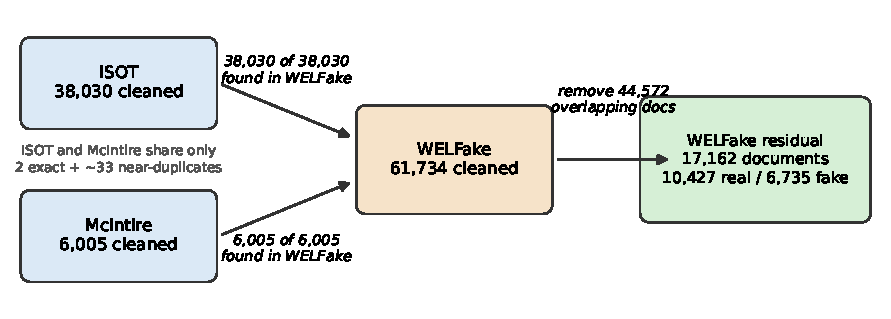
\includegraphics[width=0.86\textwidth]{fig_overlap.pdf}
\caption{Construction of the WELFake residual. Every cleaned ISOT and McIntire document has a normalized exact-text match in WELFake; ISOT and McIntire share almost no documents. WELFake documents flagged by the builder's stripped-body exact, prefix or primary near-duplicate rules are removed to leave the residual used as the third dataset. One stripped-empty exact match survives this policy, as described in the methods.}
\label{fig:overlap}
\end{figure}

\begin{table}[t]
\caption{Datasets. Raw and cleaned sizes, and the analysis set (real/fake).}
\label{tab:data}
\centering\footnotesize\setlength{\tabcolsep}{3pt}
\adjustbox{max width=\linewidth}{\begin{tabular}{@{}lrrrr@{}}
\toprule
Dataset & Raw & Cleaned & Analysis set (R/F) & Mean words (R/F)\\
\midrule
ISOT & 44,898 & 38,030 & 20,923/17,107 & 395/448\\
McIntire & 6,335 & 6,005 & 2,964/3,041 & 939/709\\
WELFake residual & 72,134 & 61,734 & 10,427/6,735 & 895/640\\
\bottomrule
\end{tabular}}
\par\vspace{2pt}\begin{minipage}{0.97\columnwidth}\scriptsize\raggedright Cleaning removed short/empty documents (1,106; 211; 1,799) and exact duplicates (5,762; 119; 8,601). Raw and cleaned sizes for the WELFake row refer to the full corpus; its analysis set is the residual, which excludes 44,572 documents that overlap ISOT or McIntire. Mean words are for title plus body.\end{minipage}
\end{table}


\subsection{Document-paired validation}\label{sec:paired}
The main intervention estimates below use the new document-paired protocol, rather than the archived condition-specific samples. All eight seeds (0--7) completed: 312 TF-IDF fits and 192 fits for each transformer, producing 2,088 evaluation rows (each fit evaluated on its own and the other two corpora). Article-selection manifests agree across all three models. Within each seed, corpus and length-matching setting, masking conditions and their random controls reuse identical training and evaluation articles. Cluster separation, sample counts and hashes passed the saved-provenance audit. This validates result completeness and recorded pairing; it does not independently repeat training, NER or the raw-text overlap audit.

\paragraph{TF-IDF: the main finding persists.}
The pooled baseline AUC gap is 0.212, falling to 0.157 under S+L+E (Table~\ref{tab:paired_conditions}). The seed-wise share removed is 26.2\% (95\% interval 24.5--27.8\%), compared with 24.7\% in the archived run. L+E alone removes 27.5\% (25.7--29.2\%). Adding source-marker masking does not increase this raw reduction; its negative matched-control contrast is consistent with the slightly smaller S+L+E reduction, without identifying a unique mechanism. These percentages are calculated within seed before averaging, not from rounded pooled gaps. Length matching raises cross-dataset AUC by 0.037 [0.033, 0.040]. Entity masking exceeds matched random deletion by 0.021 [0.019, 0.023], and retains its advantage after length matching: 0.021 [0.020, 0.022]. S+L+E exceeds its length-matched random control by 0.013 [0.012, 0.015]. All four pooled contrasts have the same sign in eight of eight seeds. Source masking falls below its random control by 0.009 [0.009, 0.010]; it does not account for the positive combined result.

\begin{table}[t]
\caption{Document-paired validation: pooled cross-dataset AUC and AUC gap (mean and 95\% interval over eight seeds). Six ordered pairs are averaged within seed.}\label{tab:paired_conditions}
\centering\footnotesize
\adjustbox{max width=\linewidth}{\begin{tabular}{@{}llcc@{}}
\toprule
Model & Condition & Cross AUC & AUC gap\\
\midrule
TF-IDF & C0 & 0.772 [0.768, 0.777] & 0.212 [0.208, 0.217]\\
TF-IDF & L+E & 0.825 [0.821, 0.830] & 0.154 [0.151, 0.157]\\
TF-IDF & S+L+E & 0.816 [0.811, 0.821] & 0.157 [0.154, 0.160]\\
TF-IDF & L+$R_E$ & 0.804 [0.800, 0.809] & 0.179 [0.176, 0.182]\\
TF-IDF & L+$R_{SE}$ & 0.803 [0.799, 0.808] & 0.180 [0.177, 0.184]\\
DistilBERT & C0 & 0.813 [0.791, 0.836] & 0.184 [0.161, 0.207]\\
DistilBERT & L+E & 0.828 [0.821, 0.835] & 0.167 [0.160, 0.174]\\
DistilBERT & S+L+E & 0.834 [0.827, 0.842] & 0.158 [0.150, 0.166]\\
DistilBERT & L+$R_E$ & 0.841 [0.832, 0.850] & 0.155 [0.147, 0.164]\\
DistilBERT & L+$R_{SE}$ & 0.842 [0.834, 0.850] & 0.154 [0.146, 0.162]\\
RoBERTa & C0 & 0.812 [0.776, 0.847] & 0.188 [0.152, 0.224]\\
RoBERTa & L+E & 0.902 [0.892, 0.913] & 0.096 [0.085, 0.107]\\
RoBERTa & S+L+E & 0.910 [0.902, 0.918] & 0.088 [0.079, 0.096]\\
RoBERTa & L+$R_E$ & 0.916 [0.908, 0.923] & 0.083 [0.076, 0.091]\\
RoBERTa & L+$R_{SE}$ & 0.900 [0.887, 0.913] & 0.099 [0.086, 0.112]\\
\bottomrule
\end{tabular}
}
\end{table}

\paragraph{Transformers: raw gains do not isolate a cue effect.}
DistilBERT entity masking performs worse than matched random deletion by 0.028 AUC [$-$0.039, $-$0.017], with negative differences in all eight seeds (Table~\ref{tab:paired_pooled}). This is clearer than the archived estimate of $-0.010$ [$-$0.025, 0.005]. With length matching the difference is $-0.013$ [$-$0.020, $-$0.005], but it does not survive the descriptive six-contrast Holm adjustment. For S+L+E the DistilBERT estimate is $-0.007$ [$-$0.018, 0.003], and for RoBERTa it is $+0.010$ [$-$0.010, 0.030]; both intervals include zero. Neither establishes equivalence. RoBERTa's E and L+E contrasts also have intervals spanning zero.

RoBERTa's S+L+E gap falls from 0.188 to 0.088, a seed-wise raw reduction of 50.8\% [39.5, 62.2\%]. Its length-matched random control already has a gap of 0.099 and cross-dataset AUC of 0.900, against 0.910 for S+L+E. Thus a large raw reduction does not establish a benefit specific to the selected cues. The focused transformer validation did not include S, S+E, $R_S$ or $R_{SE}$, so the archived $+0.102$ RoBERTa random-deletion result was not directly retested. The validation supports sensitivity to random deletion through the tested controls, rather than reproducing that exact contrast.

\begin{table}[t]
\caption{All six document-paired cross-dataset AUC contrasts in the descriptive multiplicity family: mean and 95\% interval over eight seeds. Positive values favor the first condition. L versus C0 changes article selection by design; masking comparisons within each length setting reuse identical articles. ``Not run denotes an omitted transformer contrast, assigned $p=1$ only for multiplicity adjustment (Table~\ref{tab:paired_multiplicity}).}\label{tab:paired_pooled}
\centering\scriptsize
\adjustbox{max width=\linewidth}{\begin{tabular}{@{}lccc@{}}
\toprule
Contrast & TF-IDF & DistilBERT & RoBERTa\\
\midrule
S $-$ $R_S$ & -0.009 [-0.010, -0.009] & not run & not run\\
E $-$ $R_E$ & +0.021 [+0.019, +0.023] & -0.028 [-0.039, -0.017] & -0.009 [-0.024, +0.007]\\
S+E $-$ $R_{SE}$ & +0.012 [+0.010, +0.013] & not run & not run\\
L $-$ C0 & +0.037 [+0.033, +0.040] & +0.016 [-0.003, +0.035] & -0.006 [-0.032, +0.020]\\
L+E $-$ L+$R_E$ & +0.021 [+0.020, +0.022] & -0.013 [-0.020, -0.005] & -0.013 [-0.029, +0.003]\\
S+L+E $-$ L+$R_{SE}$ & +0.013 [+0.012, +0.015] & -0.007 [-0.018, +0.003] & +0.010 [-0.010, +0.030]\\
\bottomrule
\end{tabular}
}
\end{table}

\begin{figure}[t]
\centering
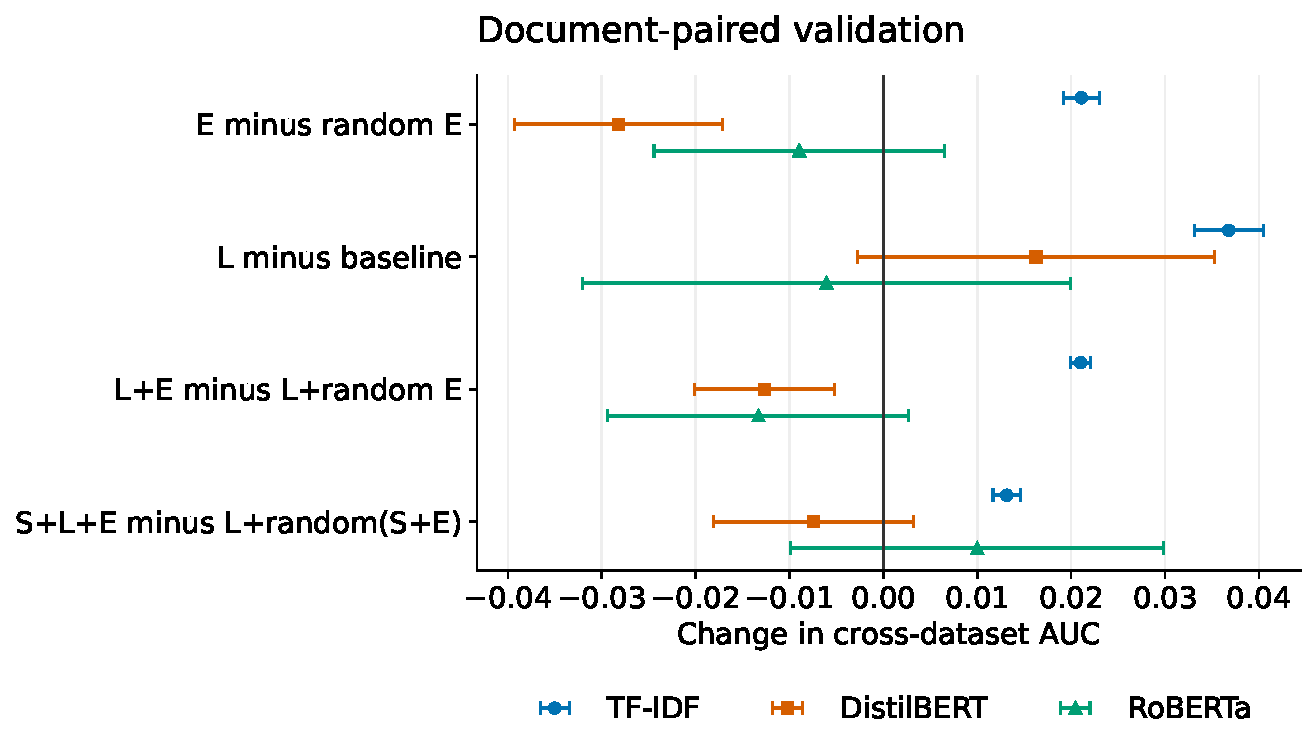
\includegraphics[width=\linewidth]{paired_validation_contrasts.pdf}
\caption{Document-paired pooled contrasts. Points and bars show means and 95\% intervals over eight seeds; the six ordered pairs are averaged within each seed. Intervals describe variability on these fixed corpora.}\label{fig:paired}
\end{figure}

\paragraph{Model differences.}
Direct seed-wise differences support a larger entity-specific effect for TF-IDF than DistilBERT: E against $R_E$ differs by 0.049 [0.038, 0.060], and L+E against L+$R_E$ differs by 0.034 [0.026, 0.041]. These model-difference estimates are descriptive and are reported in the supplement with seed values. Matching document identities across models does not make the models' optimization randomness identical.

\paragraph{Dataset-pair variation.}
Table~\ref{tab:paired_pairs} reports S+L+E against its length-matched random control. For DistilBERT, McIntire$\rightarrow$ISOT is positive (0.101 [0.074, 0.129]), all four residual-involving transfers are negative with intervals below zero, and ISOT$\rightarrow$McIntire is positive but its interval narrowly includes zero (0.028 [$-$0.0001, 0.056]). For RoBERTa, both ISOT--McIntire transfers have positive intervals, but ISOT$\rightarrow$residual is highly uncertain (0.046 [$-$0.056, 0.148]); only residual$\rightarrow$McIntire is clearly negative by its unadjusted interval. The archived claim that both transformers consistently lose against the control on residual-involving transfers is therefore not supported by the paired run. TF-IDF benefits on all four ISOT-involving transfers, whereas the McIntire--residual transfers are negative. All pair-level intervals are exploratory and unadjusted.

\begin{table}[t]
\caption{Document-paired S+L+E minus L+$R_{SE}$ by ordered pair: mean and 95\% interval over eight seeds. Exploratory; no pair-level multiplicity correction. ``Residual'' is the constructed WELFake residual.}\label{tab:paired_pairs}
\centering\scriptsize
\adjustbox{max width=\linewidth}{\begin{tabular}{@{}lccc@{}}
\toprule
Train $\rightarrow$ test & TF-IDF & DistilBERT & RoBERTa\\
\midrule
ISOT$\rightarrow$McIntire & +0.013 [+0.011, +0.015] & +0.028 [-0.000, +0.056] & +0.028 [+0.007, +0.049]\\
ISOT$\rightarrow$residual & +0.004 [+0.001, +0.007] & -0.050 [-0.075, -0.025] & +0.046 [-0.056, +0.148]\\
McIntire$\rightarrow$ISOT & +0.058 [+0.053, +0.064] & +0.101 [+0.074, +0.129] & +0.028 [+0.002, +0.054]\\
McIntire$\rightarrow$residual & -0.009 [-0.012, -0.007] & -0.017 [-0.027, -0.006] & -0.012 [-0.025, +0.001]\\
residual$\rightarrow$ISOT & +0.021 [+0.015, +0.027] & -0.077 [-0.115, -0.039] & -0.014 [-0.030, +0.002]\\
residual$\rightarrow$McIntire & -0.009 [-0.011, -0.006] & -0.031 [-0.045, -0.017] & -0.016 [-0.025, -0.006]\\
\bottomrule
\end{tabular}
}
\end{table}

\paragraph{Multiplicity and comparison with archived results.}
All six TF-IDF contrasts in the descriptive family have exact sign-flip $p=0.0078$ and Holm-adjusted $p=0.0469$. DistilBERT's E against $R_E$ has the same adjusted value; its other tested contrasts and all RoBERTa contrasts have adjusted values above 0.05. Table~\ref{tab:paired_multiplicity} lists all six contrasts, sign agreement, exact and adjusted values, including the omitted transformer contrasts assigned $p=1$. These are descriptive sensitivity summaries: the protocol was written after the original findings were known, and the seeds reuse one fixed document universe. The new run is not an independent-corpus replication or a registered confirmatory test. Archived and paired estimates are tabulated separately in the supplement. Their differences include changed sampling and recorded software versions; they cannot be attributed solely to document pairing. Appendix~\ref{sec:archived} preserves the archived factorial, exploratory and duplicate-removal results, which were not all repeated in the focused validation.

\section{External validation on Celebrity}\label{sec:external}
\subsection{Target audit and evaluation protocol}
We evaluate transfer to Celebrity, a separate web-collected fake/legitimate news collection from P\'erez-Rosas et al.~\cite{perezrosas2018automatic}. The supplied version contains 500 articles, 250 per label; it is distinct from the crowdsourced FakeNewsAMT collection in the same archive, which we do not use. The original authors describe manual checking against gossip-verification sites and other reporting. We retain their labels rather than independently adjudicating every article. Celebrity is used only as an external target, not a fourth training corpus, and its size falls below our original 3,000-per-class training-corpus threshold.

The audit compares all 500 items with every row of the frozen 61,197-document source analysis input, using normalized exact, prefix and primary/sensitivity near-duplicate checks. It records nine evidence rows involving two Celebrity articles: \texttt{062legit.txt} overlaps ISOT-12805 and \texttt{062fake.txt} overlaps WELFake-58856. Manual inspection records shared content; the ISOT/Celebrity label conflict is unresolved. A separate item, \texttt{131fake.txt}, has only one 28-word physical line and no body under our first-line-as-headline rule. We exclude provisional numeric groups 062 and 131 conservatively, retaining \textbf{496 articles, 248 per label}. Numeric groups remain provisional story links, not verified semantic pairs. No internal near-duplicate candidates meet the tested thresholds. These screens reduce detected overlap without establishing complete independence. Long articles and fact-checking/publisher-language flags are retained; a legitimate interview explicitly dates itself to 1974, so this is not a temporal holdout.

The external protocol was fixed before external scoring, after the three-corpus results were known, without formal registration. Models are retrained only on the original source corpora, retaining their configurations, seeds 0--7 and paired source selections. Every model covers C0, E, $R_E$, S+E, $R_{SE}$, L, L+E, L+$R_E$, S+L+E and L+$R_{SE}$: \textbf{240 fits per model, 720 total}. The additional S+E/$R_{SE}$ transformer pair belongs to this extension; it does not fill an omitted cell of the earlier validation. No target score is used to select hyperparameters, masking rules or checkpoints. The initial operational pilot is one job of this same frozen grid and is retained.

Primary comparisons are E minus $R_E$ and S+E minus $R_{SE}$ on all 496 eligible articles. Target IDs are fixed across seeds, source corpora and models, and random deletion matches the number of whole words removed from each document. Secondary L+E minus L+$R_E$ and S+L+E minus L+$R_{SE}$ comparisons use a separate, frozen \textbf{428-article target, 214 per label}, constructed by class-balanced length-bin sampling. These diagnostics use target labels and must not be compared with primary scores as if the target articles were identical. We report each source transfer separately, with means, sample standard deviations (SD), ranges and seed values; we introduce no external source pooling or new significance-test family. Seed variation conditions on the fixed target, not independent target samples.

\subsection{Source-specific results}
All 720 fits completed. Original source selections match all 24 saved model/seed manifests from the three-corpus study. Recorded pairing, target labels/IDs, deletion budgets, code hashes and result checksums pass verification. Independent aggregation reproduces all 288 seed/source/model AUC differences and 90 source-condition AUC summaries. These checks do not repeat training or independently recalculate metrics from per-article predictions, which were not exported. Online Resource 2 provides the saved outputs and CPU rebuild; Appendix~\ref{sec:external_appendix} gives baseline and secondary results and per-seed contrasts.

\begin{table}[t]
\caption{Celebrity primary comparisons on the fixed 496-article target: mean cross-dataset AUC difference (sample SD) across eight training seeds. Positive favors masking over matched random deletion. SD describes seed variation, not article-sampling uncertainty. Residual: constructed WELFake residual.}\label{tab:celebrity_primary}
\centering\footnotesize
\adjustbox{max width=\linewidth}{\begin{tabular}{@{}llccc@{}}
\toprule
Source & Contrast & TF-IDF & DistilBERT & RoBERTa\\
\midrule
ISOT & E $-$ $R_E$ & +0.0045 (0.0062) & -0.0176 (0.0324) & -0.0342 (0.0559)\\
ISOT & S+E $-$ $R_{SE}$ & +0.0025 (0.0044) & +0.0159 (0.0400) & -0.0033 (0.0421)\\
McIntire & E $-$ $R_E$ & +0.0095 (0.0024) & +0.0035 (0.0117) & -0.0200 (0.0176)\\
McIntire & S+E $-$ $R_{SE}$ & +0.0092 (0.0074) & +0.0205 (0.0159) & +0.0044 (0.0226)\\
Residual & E $-$ $R_E$ & +0.0164 (0.0057) & +0.0081 (0.0353) & +0.0501 (0.0283)\\
Residual & S+E $-$ $R_{SE}$ & +0.0176 (0.0086) & +0.0409 (0.0390) & +0.0665 (0.0265)\\
\bottomrule
\end{tabular}
}
\end{table}

TF-IDF's E-minus-$R_E$ means are positive from all sources (Table~\ref{tab:celebrity_primary}; Fig.~\ref{fig:celebrity_entity}). McIntire and residual means are $+0.0095$ and $+0.0164$, positive in eight of eight seeds; ISOT is smaller ($+0.0045$), positive in six of eight. This is qualified external support for the lexical-model pattern, rather than an identical effect magnitude. DistilBERT's corresponding means are $-0.0176$, $+0.0035$ and $+0.0081$ from ISOT, McIntire and the residual, with mixed signs across seeds. Its negative three-corpus pooled entity result does not transfer uniformly to Celebrity.

\begin{figure}[t]
\centering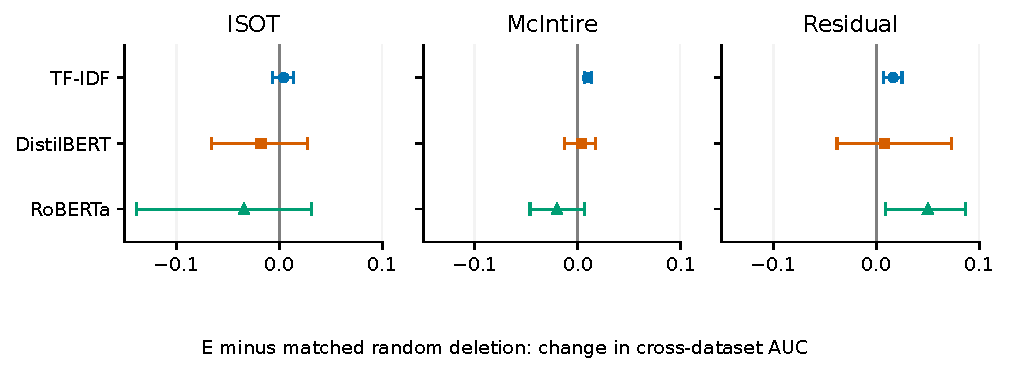
\includegraphics[width=\linewidth]{fig_celebrity_entity.pdf}
\caption{Celebrity primary E minus $R_E$ by training source. Points are means and whiskers are the observed minimum and maximum across eight seeds, \emph{not confidence intervals}. All fits use the same 496 target articles.}\label{fig:celebrity_entity}
\end{figure}

RoBERTa's primary entity means are $-0.0342$ from ISOT, $-0.0200$ from McIntire and $+0.0501$ from the residual; only the residual contrast is positive in every seed. Its primary S+E-minus-$R_{SE}$ mean from the residual is also positive in every seed ($+0.0665$). Source dependence is particularly clear in the secondary combined comparison: RoBERTa's S+L+E-minus-L+$R_{SE}$ difference is negative in all seeds from ISOT ($-0.0332$) and positive in all seeds from the residual ($+0.0866$); the McIntire mean is near zero ($+0.0011$). DistilBERT's residual-trained secondary combined contrast is positive in all seeds ($+0.0540$). These directions describe this fixed target and protocol; sign consistency alone is not a new significance claim.

Raw improvements and matched-control contrasts can point to different interpretations. For McIntire-trained RoBERTa, C0 scores 0.6521, E scores 0.7365, and $R_E$ scores 0.7566: the raw E gain is $+0.0845$, but E minus $R_E$ is $-0.0200$. Conversely, McIntire-trained TF-IDF scores 0.5835 under C0 and 0.5837 under E, despite an E-minus-$R_E$ difference of $+0.0095$. Beating random deletion need not mean beating C0. We therefore retain the original three-corpus gap estimates separately and interpret the external evidence through matched comparisons and source-specific reporting.

\section{Discussion}
The document-paired validation strengthens the central TF-IDF finding: S+L+E removes 26.2\% of its gap, and entity masking improves cross-dataset AUC beyond matched random deletion both with and without length matching. The raw gap reduction is an operational property of these interventions on these corpora, not an estimate of the maximum or unique causal contribution of the cue families. Length matching changes the sampled population and uses class labels in the target corpus, so it remains a diagnostic rather than an unlabeled deployment method.

\emph{Random controls change the transformer interpretation.} Entity masking is worse than random deletion for DistilBERT in the paired comparison, rather than merely showing an inconclusive advantage. For RoBERTa, S+L+E removes about half the raw gap but has no clear pooled benefit over its length-matched random control. This distinction prevents a large raw gain from being attributed to the selected cues without accounting for nonspecific perturbation. The focused transformer design leaves source-only contrasts untested in the new run; their archived values should not be presented as newly validated findings.

\emph{Dataset pairs remain essential.} DistilBERT's negative residual-involving contrasts persist, but the analogous RoBERTa pattern is weaker and one interval is very wide. A pooled average conceals this uncertainty. The stronger claim that both transformers benefit only on ISOT--McIntire transfers is not supported consistently by the paired validation. Pair-level results remain exploratory rather than population-level evidence about dataset types.

\emph{External transfer is source dependent.} Celebrity provides a distinct target while retaining the source-side design. TF-IDF's primary entity-minus-random mean is positive for all sources, but the transformer response changes with the source corpus. In particular, the residual-trained RoBERTa advantage contrasts with its negative ISOT- and McIntire-trained entity means. The negative pooled DistilBERT entity result from the three-corpus analysis is not universal on the external target. These are meaningful boundary conditions, not grounds to discard adverse outcomes or pool them away. Because the target is small, collection-specific and only overlap-screened, the extension broadens the empirical setting without establishing generalization to all news domains.

\emph{Deletion changes transformer inputs.} A regularization-like response is one possible explanation for random deletion gains, but deletion also shifts later content into the first 256 tokens. We did not hold the original token window fixed, match subword counts, or isolate training-side from test-side changes. The results therefore support model-dependent sensitivity to these transformations, without identifying its mechanism.

\emph{The audit and the intervention answer different questions.} Normalized overlap checks motivated construction of the WELFake residual. Reuters markers support the interpretation of label direction but do not independently verify article veracity. The paired-validation audit checks saved sample identities and result provenance; it does not substitute for reproducing normalization, duplicate matching or human label validation from the source data.

For dataset-transfer studies, these findings support reporting overlap checks, label mappings, article-paired masking comparisons, matched random controls, model-specific responses and ordered dataset pairs. Length-matching comparisons should state explicitly that they alter the sampled population. Uncertain contrasts should be described as inconclusive rather than equivalent.

\section{Limitations}
The frozen analysis input retains one fake-labelled WELFake row with an exact lightly normalized body match in ISOT: both become empty under artifact stripping and escape the builder's stripped-hash rule. Thus the residual is not completely free of exact cross-corpus overlap. Both identifiers occur in the historical exclusion list used for duplicate-removal checks. File hashes and counts establish input identity and size, not independent overlap verification or article veracity. Inspection of all saved paired-validation selection manifests found neither identifier in any training or evaluation selection across the eight seeds and three models. This finding applies to this pair and does not establish that all residual overlap has been removed.

The principal analysis covers three English news corpora dominated by 2016--2017 US politics, one lexical model and two fine-tuned transformers. The WELFake residual is constructed rather than independently collected. Dataset labels were not re-verified by human fact-checkers, and may encode source reliability rather than article-level veracity. Celebrity adds a separately collected external target after lexical overlap screening, not an independent fourth training corpus; no temporal holdout was evaluated. The paired run reuses the original document universe and eight seed identifiers, and its protocol was developed after the archived findings were known; it is a methodological validation, not an independent-data or prospectively registered confirmation.

Pairing holds article identities fixed for masking comparisons within each length-matching setting. L versus C0 changes article selection intentionally and uses target labels. Training is subsampled, and the transformers see only 256 tokens. Deletion before truncation changes input content; matching whole-word deletion counts does not match subword counts or positions. Source expressions were developed after inspecting predictive cues, and entity masking uses a small NER model. Neither transformation removes all information about its intended cue family. None establishes exclusive causal attribution.

In the three-corpus validation, only TF-IDF received the full 13-condition paired design; the transformers received eight conditions. Archived source splits, temporal masking, source-only transformer contrasts and duplicate-removal checks were not repeated with document pairing. The original duplicate-removal rerun did not cover RoBERTa or the added conditions. Saved provenance checks do not independently reproduce raw-text matching, NER or GPU training. Archived and new runs also differ in software, so changes between their estimates cannot be assigned solely to the pairing fix. Some original environment records are incomplete.

All seeds sample from one fixed universe. Seed-level intervals describe variability under this protocol, rather than uncertainty across future datasets. The six-contrast Holm summaries are descriptive because the family was chosen after earlier exploration. Pair-level analyses are unadjusted and exploratory, and the original dataset-size rule was narrowly missed.

Celebrity is small and domain-specific, with author-supplied labels and provisional numeric story groups. The audit records shared-content overlap and an unresolved cross-corpus label conflict, and one item lacks a body; group-based exclusions are conservative but cannot eliminate all semantic overlap. Fact-checking language and long historical articles remain. Target-side length matching uses labels, and its 428 articles differ from the 496-article primary target. All models share these fixed targets across seeds, so seed variability does not quantify article/story sampling uncertainty. Per-article prediction scores were not exported, preventing independent metric recalculation or a paired story bootstrap from the saved outputs. The external protocol followed earlier findings and was not formally registered; primary/secondary status is local to this extension, not a new confirmatory claim.

\section{Conclusion}
On three audited English news corpora, document-paired validation reproduces the main TF-IDF finding: source masking, length matching and entity masking together remove 26.2\% of the pooled AUC gap, and entity masking improves transfer beyond matched random deletion, including after length matching. For DistilBERT, entity masking performs worse than matched random deletion. Neither transformer has an established positive pooled benefit of S+L+E over its length-matched random control, despite RoBERTa's large raw gap reduction. Dataset-pair effects vary, and the archived transformer pattern is not uniformly supported by the paired run. Artifact-removal gains should therefore be interpreted through document-paired controls and pair-level reporting, with conclusions restricted to the tested corpora and transformations.

\section{Future work}
\emph{Immediate extensions:} more datasets, including ones with different construction, languages and years; temporally disjoint splits; an independently collected corpus to replace the constructed WELFake residual; and further transformer architectures. \emph{Methodological extensions:} learned or human-validated source-marker detection in place of regular expressions; separating publisher-type signal from veracity signal; counterfactual rewriting as a causal intervention; and evaluation with human-verified labels and instruction-tuned LLMs.



\section*{Declarations}
\bmhead{Funding} Not applicable.
\bmhead{Competing interests} The authors declare that they have no competing interests.
\bmhead{Ethics approval} Not applicable. The study uses public news corpora and involves no human participants or personal data collected by the authors.
\bmhead{Consent to participate and to publish} Not applicable.
\bmhead{Data availability} The datasets are public and are not redistributed by the authors. The copies used were downloaded from Kaggle for ISOT (\url{https://www.kaggle.com/datasets/rahulogoel/isot-fake-news-dataset}) and WELFake (\url{https://www.kaggle.com/datasets/studymart/welfake-dataset-for-fake-news}) and from a GitHub mirror for McIntire (\url{https://github.com/joolsa/fake_real_news_dataset}, file \texttt{fake\_or\_real\_news.csv}, 6,335 articles); the original publications are cited in Section~\ref{sec:data}. The document identifiers of the flagged duplicates, the per-cell result files, the configuration files and the seeds are provided in the code repository. \todo{VERIFY: the repository must not track dataset-derived files (the McIntire CSV and the overlap-pair files) if this statement is kept.}
\bmhead{Code availability} Code for the audit, interventions, experiments and analysis: \url{https://github.com/abiroh-p/ERM}.
\bmhead{Computing environment and software} The TF-IDF arm was run on the first author's own computer (Lenovo 81X8, x64, Intel64 Family 6 Model 140 processor, CPU only) with NumPy 2.3.2, pandas 2.3.3, scikit-learn 1.8.0, SciPy 1.16.3, Matplotlib 3.10.0, spaCy 3.8.16 with the \texttt{en\_core\_web\_sm} model 3.8.0 and Python 3.12.4. \todo{VERIFY: confirm these versions in the local environment with the command given in the reply.} The archived DistilBERT runs used a Google Colab NVIDIA Tesla T4 GPU; the library versions of that session were not recorded. The added conditions, the RoBERTa arm and the reproduction check were run on Kaggle with two NVIDIA T4 GPUs (Python 3.12.13, PyTorch 2.10.0+cu128, Transformers 5.0.0); each such run stores its arguments and library versions next to its results.
% Earlier draft also listed PyTorch 2.11.0 (CUDA 13.0, cuDNN 9.27), Transformers 5.17.0 and Tokenizers 0.23.2; these cannot be attributed to any recorded run and were removed. Re-add only with evidence.
\bmhead{Author contributions} Abishek Prasad: conceptualization, methodology, software, validation, formal analysis, investigation, data curation, writing -- original draft, writing -- review and editing. Natasha Rai: conceptualization, methodology, writing -- original draft, writing -- review and editing, visualization, supervision.
\bmhead{Acknowledgements} The authors used an AI assistant (Anthropic's Claude) to help develop and debug analysis code, to draft and edit parts of the text, and to check bibliographic details. The authors ran all experiments, checked the reported results against the released code and result files, and take full responsibility for the content of the paper.

\FloatBarrier
\appendix
\section{Document-paired inference and seed results}
For each seed, cross-dataset AUC contrasts are first computed within each ordered corpus pair and then averaged over the six pairs. The reported mean and 95\% $t$-interval use the resulting eight values. Seeds are the repeated unit; the six transfers within a seed are not independent samples. Exact sign-flip values enumerate the 256 sign assignments; with eight seeds the smallest two-sided value is 0.0078125. Holm correction retains the six contrasts in the descriptive family per model and outcome, assigning $p=1$ to the two unrun transformer contrasts. This is a descriptive analysis of a fixed document universe, informed by earlier exploration. Failure to reject zero is not evidence of equivalence.


\begin{table}[htbp]
\caption{Complete document-paired cross-dataset AUC multiplicity summary. Sign agreement counts seed-level differences with the same sign as their mean, after averaging the six ordered pairs within seed. Holm correction is applied separately within each model's six-contrast AUC family. Asterisk: an unrun contrast contributes $p=1$ to correction only; no effect or sign-flip test is estimated. These post-exploration summaries are descriptive.}\label{tab:paired_multiplicity}
\centering\footnotesize
\adjustbox{max width=\linewidth}{\begin{tabular}{@{}llccc@{}}
\toprule
Model & Contrast & Sign agreement & Exact $p$ & Holm $p$\\
\midrule
TF-IDF & S $-$ $R_S$ & 8/8 & 0.0078 & 0.0469\\
TF-IDF & E $-$ $R_E$ & 8/8 & 0.0078 & 0.0469\\
TF-IDF & S+E $-$ $R_{SE}$ & 8/8 & 0.0078 & 0.0469\\
TF-IDF & L $-$ C0 & 8/8 & 0.0078 & 0.0469\\
TF-IDF & L+E $-$ L+$R_E$ & 8/8 & 0.0078 & 0.0469\\
TF-IDF & S+L+E $-$ L+$R_{SE}$ & 8/8 & 0.0078 & 0.0469\\
DistilBERT & S $-$ $R_S$ & not run & -- & 1.0000*\\
DistilBERT & E $-$ $R_E$ & 8/8 & 0.0078 & 0.0469\\
DistilBERT & S+E $-$ $R_{SE}$ & not run & -- & 1.0000*\\
DistilBERT & L $-$ C0 & 5/8 & 0.0938 & 0.3750\\
DistilBERT & L+E $-$ L+$R_E$ & 7/8 & 0.0234 & 0.1172\\
DistilBERT & S+L+E $-$ L+$R_{SE}$ & 6/8 & 0.1250 & 0.3750\\
RoBERTa & S $-$ $R_S$ & not run & -- & 1.0000*\\
RoBERTa & E $-$ $R_E$ & 6/8 & 0.1953 & 0.9766\\
RoBERTa & S+E $-$ $R_{SE}$ & not run & -- & 1.0000*\\
RoBERTa & L $-$ C0 & 5/8 & 0.5781 & 1.0000\\
RoBERTa & L+E $-$ L+$R_E$ & 7/8 & 0.1016 & 0.6094\\
RoBERTa & S+L+E $-$ L+$R_{SE}$ & 6/8 & 0.2812 & 1.0000\\
\bottomrule
\end{tabular}
}
\end{table}

\begin{table}[htbp]
\caption{Document-paired model differences: TF-IDF minus DistilBERT in each pooled AUC contrast (mean, 95\% interval and sign agreement across eight seeds). Exploratory.}\label{tab:paired_model_diff}
\centering\scriptsize
\adjustbox{max width=\linewidth}{\begin{tabular}{@{}lcc@{}}
\toprule
Contrast & TF-IDF $-$ DistilBERT & Sign agreement\\
\midrule
E $-$ $R_E$ & +0.049 [+0.038, +0.060] & 8/8\\
L $-$ C0 & +0.021 [+0.003, +0.038] & 7/8\\
L+E $-$ L+$R_E$ & +0.034 [+0.026, +0.041] & 8/8\\
S+L+E $-$ L+$R_{SE}$ & +0.021 [+0.010, +0.032] & 7/8\\
\bottomrule
\end{tabular}
}
\end{table}

\begin{table}[htbp]
\caption{Document-paired TF-IDF: per-seed cross-dataset AUC contrasts, averaging six ordered pairs within each seed. Full precision is supplied in the result archive.}
\centering\scriptsize
\adjustbox{max width=\linewidth}{\begin{tabular}{@{}rcccc@{}}
\toprule
Seed & E $-$ $R_E$ & L $-$ C0 & L+E $-$ L+$R_E$ & S+L+E $-$ L+$R_{SE}$\\
\midrule
0 & +0.019 & +0.038 & +0.022 & +0.014\\
1 & +0.022 & +0.034 & +0.020 & +0.011\\
2 & +0.024 & +0.040 & +0.022 & +0.015\\
3 & +0.018 & +0.040 & +0.020 & +0.013\\
4 & +0.023 & +0.031 & +0.022 & +0.016\\
5 & +0.024 & +0.038 & +0.020 & +0.013\\
6 & +0.020 & +0.031 & +0.019 & +0.011\\
7 & +0.019 & +0.043 & +0.023 & +0.012\\
\bottomrule
\end{tabular}
}
\end{table}

\begin{table}[htbp]
\caption{Document-paired DistilBERT: per-seed cross-dataset AUC contrasts, averaging six ordered pairs within each seed. Full precision is supplied in the result archive.}
\centering\scriptsize
\adjustbox{max width=\linewidth}{\begin{tabular}{@{}rcccc@{}}
\toprule
Seed & E $-$ $R_E$ & L $-$ C0 & L+E $-$ L+$R_E$ & S+L+E $-$ L+$R_{SE}$\\
\midrule
0 & -0.019 & -0.002 & -0.016 & -0.001\\
1 & -0.036 & -0.003 & -0.019 & -0.026\\
2 & -0.044 & +0.040 & -0.020 & -0.014\\
3 & -0.036 & +0.028 & -0.021 & -0.005\\
4 & -0.010 & +0.018 & -0.016 & -0.013\\
5 & -0.013 & -0.012 & -0.003 & -0.018\\
6 & -0.043 & +0.008 & -0.011 & +0.004\\
7 & -0.024 & +0.053 & +0.004 & +0.013\\
\bottomrule
\end{tabular}
}
\end{table}

\begin{table}[htbp]
\caption{Document-paired RoBERTa: per-seed cross-dataset AUC contrasts, averaging six ordered pairs within each seed. Full precision is supplied in the result archive.}
\centering\scriptsize
\adjustbox{max width=\linewidth}{\begin{tabular}{@{}rcccc@{}}
\toprule
Seed & E $-$ $R_E$ & L $-$ C0 & L+E $-$ L+$R_E$ & S+L+E $-$ L+$R_{SE}$\\
\midrule
0 & -0.006 & +0.031 & -0.027 & -0.023\\
1 & -0.025 & -0.027 & +0.020 & +0.039\\
2 & -0.010 & +0.032 & -0.018 & -0.021\\
3 & -0.024 & -0.045 & -0.042 & +0.039\\
4 & +0.005 & +0.026 & -0.023 & +0.020\\
5 & +0.027 & -0.014 & -0.000 & +0.005\\
6 & -0.030 & -0.017 & -0.015 & +0.006\\
7 & -0.008 & -0.035 & -0.001 & +0.016\\
\bottomrule
\end{tabular}
}
\end{table}

\FloatBarrier
\section{Celebrity external-validation details}\label{sec:external_appendix}
The following tables concern Celebrity only and are not pooled with the three-corpus transfers. Baseline AUC uses the fixed 496-article primary target. Secondary contrasts use the separate 428-article length-matched target and target labels. Parenthesized SD describes variability across eight training/random-deletion seeds; it is not a confidence interval. All per-seed contrasts are differences in cross-dataset AUC under the frozen external protocol. Source and target identities are paired within each comparison. Full-precision metrics, all job records, target selections and provenance accompany Online Resource 2.

\begin{table}[htbp]
\caption{Celebrity baseline (C0) cross-dataset AUC: mean (sample SD) across eight seeds on the 496-article target.}\label{tab:celebrity_baselines}
\centering\footnotesize\adjustbox{max width=\linewidth}{\begin{tabular}{@{}lccc@{}}
\toprule
Source & TF-IDF & DistilBERT & RoBERTa\\
\midrule
ISOT & 0.5533 (0.0034) & 0.6035 (0.0404) & 0.6865 (0.0203)\\
McIntire & 0.5835 (0.0033) & 0.6063 (0.0130) & 0.6521 (0.0336)\\
Residual & 0.6853 (0.0055) & 0.6330 (0.0285) & 0.5992 (0.0314)\\
\bottomrule
\end{tabular}
}
\end{table}

\begin{table}[htbp]
\caption{Celebrity secondary diagnostics on the 428-article length-matched target: mean AUC difference (sample SD) across eight seeds. Positive favors masking over the matched length-plus-random-deletion control. No comparison with the primary target is implied.}\label{tab:celebrity_secondary}
\centering\footnotesize\adjustbox{max width=\linewidth}{\begin{tabular}{@{}llccc@{}}
\toprule
Source & Contrast & TF-IDF & DistilBERT & RoBERTa\\
\midrule
ISOT & L+E $-$ L+$R_E$ & +0.0025 (0.0036) & -0.0295 (0.0606) & -0.0395 (0.0307)\\
ISOT & S+L+E $-$ L+$R_{SE}$ & +0.0006 (0.0042) & -0.0090 (0.0457) & -0.0332 (0.0182)\\
McIntire & L+E $-$ L+$R_E$ & +0.0144 (0.0079) & +0.0125 (0.0189) & -0.0021 (0.0183)\\
McIntire & S+L+E $-$ L+$R_{SE}$ & +0.0078 (0.0061) & +0.0145 (0.0242) & +0.0011 (0.0298)\\
Residual & L+E $-$ L+$R_E$ & +0.0143 (0.0069) & +0.0193 (0.0188) & +0.0678 (0.0454)\\
Residual & S+L+E $-$ L+$R_{SE}$ & +0.0146 (0.0070) & +0.0540 (0.0202) & +0.0866 (0.0267)\\
\bottomrule
\end{tabular}
}
\end{table}

\begin{table}[htbp]
\caption{Celebrity TF-IDF per-seed AUC contrasts by training source. First two contrasts: primary (496 articles); last two: secondary (428 articles). Residual: WELFake residual.}
\centering\scriptsize\adjustbox{max width=\linewidth}{\begin{tabular}{@{}lrcccc@{}}
\toprule
Source & Seed & E $-$ $R_E$ & S+E $-$ $R_{SE}$ & L+E $-$ L+$R_E$ & S+L+E $-$ L+$R_{SE}$\\
\midrule
ISOT & 0 & +0.0136 & +0.0033 & +0.0054 & -0.0007\\
ISOT & 1 & -0.0061 & -0.0015 & +0.0006 & -0.0016\\
ISOT & 2 & +0.0037 & -0.0020 & -0.0021 & -0.0019\\
ISOT & 3 & -0.0013 & +0.0028 & -0.0006 & +0.0019\\
ISOT & 4 & +0.0038 & +0.0026 & +0.0024 & +0.0028\\
ISOT & 5 & +0.0083 & +0.0120 & +0.0004 & +0.0077\\
ISOT & 6 & +0.0049 & +0.0030 & +0.0077 & +0.0029\\
ISOT & 7 & +0.0090 & -0.0004 & +0.0064 & -0.0064\\
McIntire & 0 & +0.0064 & +0.0110 & +0.0072 & +0.0113\\
McIntire & 1 & +0.0087 & +0.0019 & +0.0275 & +0.0034\\
McIntire & 2 & +0.0082 & +0.0142 & +0.0210 & +0.0185\\
McIntire & 3 & +0.0115 & +0.0141 & +0.0174 & +0.0106\\
McIntire & 4 & +0.0134 & +0.0031 & +0.0166 & +0.0009\\
McIntire & 5 & +0.0074 & -0.0010 & +0.0026 & +0.0011\\
McIntire & 6 & +0.0092 & +0.0097 & +0.0126 & +0.0053\\
McIntire & 7 & +0.0112 & +0.0207 & +0.0103 & +0.0110\\
Residual & 0 & +0.0071 & +0.0034 & +0.0074 & +0.0154\\
Residual & 1 & +0.0179 & +0.0247 & +0.0186 & +0.0121\\
Residual & 2 & +0.0162 & +0.0130 & +0.0112 & +0.0085\\
Residual & 3 & +0.0134 & +0.0264 & +0.0041 & +0.0123\\
Residual & 4 & +0.0250 & +0.0176 & +0.0239 & +0.0162\\
Residual & 5 & +0.0231 & +0.0150 & +0.0199 & +0.0186\\
Residual & 6 & +0.0139 & +0.0119 & +0.0107 & +0.0053\\
Residual & 7 & +0.0143 & +0.0292 & +0.0183 & +0.0283\\
\bottomrule
\end{tabular}
}
\end{table}

\begin{table}[htbp]
\caption{Celebrity DistilBERT per-seed AUC contrasts by training source. First two contrasts: primary (496 articles); last two: secondary (428 articles).}
\centering\scriptsize\adjustbox{max width=\linewidth}{\begin{tabular}{@{}lrcccc@{}}
\toprule
Source & Seed & E $-$ $R_E$ & S+E $-$ $R_{SE}$ & L+E $-$ L+$R_E$ & S+L+E $-$ L+$R_{SE}$\\
\midrule
ISOT & 0 & -0.0654 & +0.0093 & -0.0432 & -0.0619\\
ISOT & 1 & +0.0036 & +0.0503 & -0.1341 & +0.0069\\
ISOT & 2 & -0.0123 & -0.0261 & -0.0553 & -0.0157\\
ISOT & 3 & -0.0542 & -0.0504 & -0.0173 & -0.0145\\
ISOT & 4 & -0.0152 & +0.0627 & +0.0862 & +0.0854\\
ISOT & 5 & -0.0368 & +0.0499 & -0.0298 & -0.0145\\
ISOT & 6 & +0.0114 & +0.0313 & -0.0317 & -0.0586\\
ISOT & 7 & +0.0277 & +0.0005 & -0.0106 & +0.0010\\
McIntire & 0 & -0.0128 & +0.0038 & +0.0255 & +0.0302\\
McIntire & 1 & +0.0162 & +0.0184 & +0.0420 & +0.0536\\
McIntire & 2 & +0.0040 & -0.0065 & -0.0124 & +0.0297\\
McIntire & 3 & +0.0129 & +0.0346 & +0.0180 & +0.0194\\
McIntire & 4 & +0.0170 & +0.0407 & +0.0198 & +0.0098\\
McIntire & 5 & +0.0027 & +0.0280 & +0.0022 & -0.0097\\
McIntire & 6 & +0.0004 & +0.0161 & -0.0124 & -0.0229\\
McIntire & 7 & -0.0124 & +0.0294 & +0.0173 & +0.0063\\
Residual & 0 & -0.0186 & +0.0526 & +0.0063 & +0.0589\\
Residual & 1 & +0.0094 & +0.0317 & +0.0272 & +0.0737\\
Residual & 2 & -0.0381 & +0.0023 & +0.0076 & +0.0319\\
Residual & 3 & +0.0733 & +0.1199 & +0.0168 & +0.0804\\
Residual & 4 & +0.0169 & +0.0626 & +0.0383 & +0.0290\\
Residual & 5 & -0.0178 & -0.0009 & -0.0103 & +0.0320\\
Residual & 6 & +0.0026 & +0.0194 & +0.0195 & +0.0643\\
Residual & 7 & +0.0368 & +0.0398 & +0.0488 & +0.0614\\
\bottomrule
\end{tabular}
}
\end{table}

\begin{table}[htbp]
\caption{Celebrity RoBERTa per-seed AUC contrasts by training source. First two contrasts: primary (496 articles); last two: secondary (428 articles). No article-level sampling intervals are estimated.}
\centering\scriptsize\adjustbox{max width=\linewidth}{\begin{tabular}{@{}lrcccc@{}}
\toprule
Source & Seed & E $-$ $R_E$ & S+E $-$ $R_{SE}$ & L+E $-$ L+$R_E$ & S+L+E $-$ L+$R_{SE}$\\
\midrule
ISOT & 0 & +0.0310 & +0.0508 & -0.0141 & -0.0322\\
ISOT & 1 & -0.1383 & -0.0052 & -0.0188 & -0.0660\\
ISOT & 2 & +0.0055 & +0.0361 & -0.0846 & -0.0489\\
ISOT & 3 & +0.0027 & -0.0559 & -0.0287 & -0.0324\\
ISOT & 4 & -0.0532 & -0.0288 & -0.0362 & -0.0142\\
ISOT & 5 & -0.0876 & -0.0519 & -0.0354 & -0.0360\\
ISOT & 6 & -0.0141 & +0.0420 & -0.0091 & -0.0275\\
ISOT & 7 & -0.0192 & -0.0137 & -0.0888 & -0.0087\\
McIntire & 0 & +0.0064 & -0.0085 & -0.0145 & +0.0324\\
McIntire & 1 & -0.0090 & +0.0201 & -0.0056 & +0.0064\\
McIntire & 2 & -0.0041 & -0.0342 & +0.0012 & -0.0240\\
McIntire & 3 & -0.0310 & +0.0345 & +0.0379 & +0.0552\\
McIntire & 4 & -0.0463 & +0.0085 & -0.0117 & -0.0003\\
McIntire & 5 & -0.0147 & -0.0172 & -0.0226 & -0.0260\\
McIntire & 6 & -0.0349 & +0.0163 & +0.0044 & -0.0074\\
McIntire & 7 & -0.0266 & +0.0160 & -0.0058 & -0.0276\\
Residual & 0 & +0.0337 & +0.0591 & +0.0609 & +0.0967\\
Residual & 1 & +0.0235 & +0.0253 & +0.1507 & +0.0823\\
Residual & 2 & +0.0093 & +0.0697 & +0.0283 & +0.0744\\
Residual & 3 & +0.0599 & +0.0939 & +0.0881 & +0.1039\\
Residual & 4 & +0.0360 & +0.0728 & +0.1054 & +0.1308\\
Residual & 5 & +0.0768 & +0.0431 & +0.0158 & +0.0374\\
Residual & 6 & +0.0744 & +0.0595 & +0.0631 & +0.0876\\
Residual & 7 & +0.0868 & +0.1086 & +0.0305 & +0.0799\\
\bottomrule
\end{tabular}
}
\end{table}
\FloatBarrier

\FloatBarrier
\section{Archived experiments}\label{sec:archived}
The following results retain the original condition-specific sampling protocol. They are reported for transparency and historical comparison, not pooled with the document-paired validation. Sample sizes match across archived conditions but article identities generally differ. All numbers, figures and inferential summaries in this appendix refer to the archived protocol. Statements such as ``same samples'' in the model description mean shared across models for a given condition, not shared across conditions. The main results and conclusions use Section~\ref{sec:paired}. The exploratory source split, temporal masking and duplicate-removal check were not repeated with paired sampling.

\subsection{TF-IDF: pooled results}
Table~\ref{tab:pooled} and Fig.~\ref{fig:gap} give the pooled results. The baseline AUC gap is 0.213. Applying all three interventions gives 0.160, which removes 24.7\% of the gap (95\% interval 21.6--27.8\%; computed per seed and averaged, not from the rounded pooled gaps). The reduction comes from length matching and entity masking: L+E alone removes 27.3\% (24.8--29.7\%), slightly more than all three together, because source masking does not reduce the gap (its estimated contribution is $-2.3\%$ \ci{-4.9}{0.3}) and slightly lowers transfer. Random-deletion controls do not reduce the gap either: it stays at 0.212--0.223 against a baseline of 0.213, and $R_E$ and $R_{SE}$ lower cross-dataset AUC by about 0.006 and 0.011. The factorial effects on the AUC gap (Table~\ref{tab:effects}) are $-0.036$ for L and $-0.022$ for E, with interactions of at most 0.002 in magnitude, so the effects are close to additive. Length matching raises cross-dataset AUC from 0.772 to 0.806 while leaving in-domain AUC unchanged (0.985): the gap shrinks because transfer improves, not because in-domain performance falls.

Against matched random deletion, entity masking raises cross-dataset AUC by 0.020 \ci{0.016}{0.024} and changes the gap by $-0.025$ \ci{-0.028}{-0.022}. Source masking has the opposite effect: cross-dataset AUC changes by $-0.014$ \ci{-0.019}{-0.009} and the gap grows by 0.006 \ci{0.001}{0.011}. Both comparisons have the same sign in all eight seeds.

\begin{table}[t]
\caption{Archived protocol: TF-IDF + LR, pooled over the six ordered pairs, eight seeds. In-domain AUC, cross-dataset AUC and AUC gap with 95\% intervals over seeds.}
\label{tab:pooled}
\centering\footnotesize
\adjustbox{max width=\linewidth}{\begin{tabular}{@{}lccc@{}}
\toprule
Condition & In AUC & Cross AUC & Gap\\
\midrule
C0 (baseline) & 0.985 & 0.772 \ci{.770}{.775} & 0.213 \ci{.210}{.216}\\
S & 0.977 & 0.760 \ci{.755}{.764} & 0.218 \ci{.214}{.221}\\
L & 0.985 & 0.806 \ci{.802}{.811} & 0.179 \ci{.174}{.183}\\
E & 0.978 & 0.786 \ci{.783}{.788} & 0.192 \ci{.190}{.195}\\
S+L & 0.978 & 0.799 \ci{.795}{.804} & 0.179 \ci{.174}{.183}\\
S+E & 0.971 & 0.777 \ci{.772}{.781} & 0.194 \ci{.189}{.199}\\
L+E & 0.980 & 0.825 \ci{.821}{.829} & 0.155 \ci{.150}{.160}\\
S+L+E & 0.974 & 0.813 \ci{.809}{.817} & 0.160 \ci{.154}{.166}\\
\midrule
$R_S$ & 0.985 & 0.774 \ci{.771}{.776} & 0.212 \ci{.209}{.214}\\
$R_E$ & 0.983 & 0.766 \ci{.763}{.769} & 0.217 \ci{.215}{.220}\\
$R_{SE}$ & 0.983 & 0.761 \ci{.757}{.764} & 0.223 \ci{.219}{.226}\\
\bottomrule
\end{tabular}}
\end{table}

\begin{figure}[t]
\centering
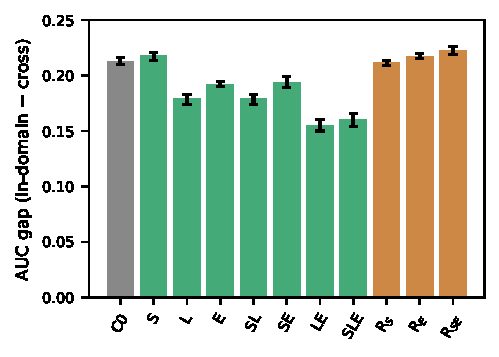
\includegraphics[width=0.78\columnwidth]{fig_gap.pdf}
\caption{Archived protocol: Pooled AUC gap by condition for TF-IDF + LR (mean, 95\% interval over eight seeds). Gray: baseline; green: factorial cells; orange: random-deletion controls. S: source-marker masking, L: length matching, E: entity masking; $R_x$: random deletion matched to $x$.}
\label{fig:gap}
\end{figure}

\begin{table}[t]
\caption{Archived protocol: TF-IDF factorial effects (coded $\pm1$) on cross-dataset AUC and on the AUC gap, 95\% intervals over eight seeds.}
\label{tab:effects}
\centering\footnotesize
\adjustbox{max width=\linewidth}{\begin{tabular}{@{}lcc@{}}
\toprule
Term & Cross AUC & AUC gap\\
\midrule
S & $-0.010$ \ci{-.012}{-.008} & $+0.003$ \ci{-.000}{.006}\\
L & $+0.037$ \ci{.036}{.039} & $-0.036$ \ci{-.038}{-.034}\\
E & $+0.016$ \ci{.012}{.020} & $-0.022$ \ci{-.026}{-.018}\\
S$\times$L & $+0.001$ \ci{-.002}{.004} & $-0.000$ \ci{-.003}{.003}\\
S$\times$E & $-0.000$ \ci{-.002}{.002} & $+0.001$ \ci{-.001}{.002}\\
L$\times$E & $+0.001$ \ci{-.002}{.003} & $+0.001$ \ci{-.002}{.003}\\
S$\times$L$\times$E & $-0.002$ \ci{-.005}{.000} & $+0.002$ \ci{-.000}{.005}\\
\bottomrule
\end{tabular}}
\end{table}

\subsection{Effects differ by dataset pair}
\begin{table}[t]
\caption{Archived protocol: TF-IDF + LR: change in cross-dataset AUC relative to the baseline, per ordered pair (mean over eight seeds; \textbf{bold}: 95\% interval over seeds excludes zero). The first column is the baseline AUC.}
\label{tab:pairs}
\centering\footnotesize
\adjustbox{max width=\linewidth}{\begin{tabular}{@{}lccccccc@{}}
\toprule
Pair (train$\rightarrow$test) & C0 AUC & S & L & E & L+E & S+L+E & $R_E$\\
\midrule
ISOT$\rightarrow$McIntire & .622 & $-.014$ & \textbf{+.055} & \textbf{+.015} & \textbf{+.072} & \textbf{+.065} & +.002\\\\
ISOT$\rightarrow$residual & .632 & $-.003$ & \textbf{+.036} & $-.003$ & \textbf{+.039} & \textbf{+.040} & $-.004$\\\\
McIntire$\rightarrow$ISOT & .738 & $\mathbf{-.040}$ & \textbf{+.069} & \textbf{+.055} & \textbf{+.141} & \textbf{+.115} & $\mathbf{-.017}$\\\\
McIntire$\rightarrow$residual & .915 & $-.009$ & $\mathbf{-.012}$ & $-.007$ & $\mathbf{-.019}$ & $\mathbf{-.023}$ & $-.002$\\\\
residual$\rightarrow$ISOT & .804 & $-.005$ & \textbf{+.075} & \textbf{+.022} & \textbf{+.098} & \textbf{+.083} & $-.013$\\\\
residual$\rightarrow$McIntire & .923 & $-.006$ & $\mathbf{-.020}$ & $-.002$ & $\mathbf{-.015}$ & $\mathbf{-.033}$ & $-.007$\\\\
\bottomrule
\end{tabular}}
\end{table}

Table~\ref{tab:pairs} and Fig.~\ref{fig:heat} show that the pooled picture hides large differences between pairs. Length matching and entity masking raise cross-dataset AUC for all four transfers involving ISOT (L+E: $+0.039$ to $+0.141$). For the two transfers between McIntire and the residual, which already start from high AUC (0.915--0.923), length matching and L+E \emph{lower} AUC slightly (L: $-0.012$ and $-0.020$; L+E: $-0.019$ and $-0.015$; all four intervals exclude zero). This matches the direction of the length confound: in ISOT the fake articles are longer (448 vs.\ 395 words on average), whereas in McIntire and the residual the real ones are (939 vs.\ 709; 895 vs.\ 640). A length cue learned on ISOT misleads on the other two datasets, whereas a cue learned on McIntire transfers to the residual because they share its direction. The pooled gain is therefore driven by ISOT-involving pairs. ISOT-trained models remain weak even after masking (cross AUC 0.67--0.69 for S+L+E), so most of the unexplained gap lies in transfers from ISOT.

\begin{figure}[t]
\centering
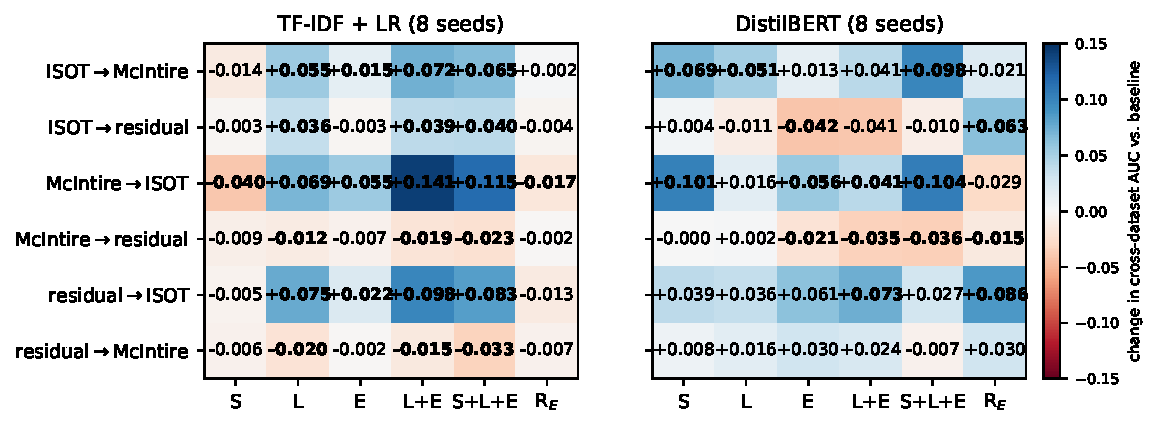
\includegraphics[width=0.92\textwidth]{fig_heatmap.pdf}
\caption{Archived protocol: Change in cross-dataset AUC relative to the baseline for each ordered pair (train $\rightarrow$ test) and intervention (TF-IDF + LR left, DistilBERT right; eight seeds each). S: source-marker masking, L: length matching, E: entity masking, combinations joined by +; $R_E$: random deletion matched to E. Bold: 95\% interval over seeds excludes zero. ``residual'' denotes the WELFake residual, and both panels share one colour scale.}
\label{fig:heat}
\end{figure}

\subsection{Exploratory analyses: source split and temporal expressions}
Table~\ref{tab:expl} reports two post-hoc analyses. Splitting S shows that the harm comes from the web-boilerplate part (share prompts, advertisements, credits, embeds, URLs): its removal changes cross-dataset AUC by $-0.014$ \ci{-0.019}{-0.010} (all eight seeds) and widens the gap by 0.009, whereas removing wire/outlet markers is neutral. A plausible reading is that such boilerplate is shared across low-quality sites and therefore transfers; it is an artifact for content-based judgement but a genuine signal of publisher type. Removing temporal expressions does not help either: it lowers cross-dataset AUC by 0.014 (eight of eight seeds; 0.012 below a size-matched random deletion), and S+L+E+T is 0.013 below S+L+E. We had expected a collection-window artifact to drive McIntire--residual transfer; the data do not support that. Both analyses are exploratory.

\begin{table}[t]
\caption{Archived protocol: Exploratory TF-IDF analyses: change in cross-dataset AUC vs.\ the baseline and vs.\ a random-deletion control of the same size, and change in AUC gap vs.\ baseline (95\% intervals over seeds).}
\label{tab:expl}
\centering\footnotesize
\adjustbox{max width=\linewidth}{\begin{tabular}{@{}lccc@{}}
\toprule
Intervention & $\Delta$AUC vs C0 & $\Delta$AUC vs random & $\Delta$gap vs C0\\
\midrule
S$_W$ (wire/outlet) & $-.000$ \ci{-.004}{.003} & $+.006$ \ci{.003}{.008} & $-.003$ \ci{-.006}{.000}\\
S$_B$ (web boilerplate) & $-.014$ \ci{-.019}{-.010} & $-.013$ \ci{-.019}{-.007} & $+.009$ \ci{.005}{.013}\\
T (temporal) & $-.014$ \ci{-.018}{-.009} & $-.012$ \ci{-.019}{-.004} & $+.011$ \ci{.005}{.016}\\
\bottomrule
\end{tabular}}
\end{table}

\subsection{Robustness to residual duplicates}
\label{sec:robust}
We flagged 207 of 61,197 documents in the analysis set that were exact, prefix or near-duplicates of a document in another dataset, or that were near-empty after stripping source markers (ISOT 63, residual 144; McIntire none, by construction). Of these, 94 of 22,005 fell in the sampling universe (0.43\%). We reran the baseline, the key interventions and the random controls without them, on all eight seeds, for both models, and compared each pooled and pair-level estimate with the main run.

\emph{TF-IDF} (baseline, L, E, L+E, $R_E$, $R_{SE}$). The pooled baseline cross-dataset AUC went from 0.772 to 0.773, and the effects of L ($+0.034$ in both runs), E ($+0.013$ to $+0.014$), L+E ($+0.053$ to $+0.054$) and E against its random control ($+0.020$ in both runs) changed by at most 0.001 \ci{-0.003}{0.006}; the AUC gaps changed by at most 0.002. None of the 24 pair-level effects changed sign, the largest absolute change was 0.012 (length matching, residual$\rightarrow$ISOT), and the median was 0.003. These changes are smaller than the seed-to-seed standard deviation of the effects themselves (0.003--0.007).

\emph{DistilBERT} (baseline, L, E, L+E, S+L+E). The pooled baseline went from 0.805 to 0.806, and the pooled effects changed by at most 0.004 (L: $+0.018$ to $+0.014$; E: $+0.016$ to $+0.015$; L+E: $+0.017$ to $+0.019$; S+L+E: $+0.029$ to $+0.026$), with all intervals for the change spanning roughly $\pm0.02$ to $\pm0.04$; the AUC gaps changed by at most 0.004. Three of the 24 pair-level effects changed sign: length matching on ISOT$\rightarrow$residual ($-0.011$ to $+0.024$) and on residual$\rightarrow$ISOT ($+0.036$ to $-0.026$), and S+L+E on ISOT$\rightarrow$residual ($-0.010$ to $+0.001$). All three involve cells whose original effect was close to zero or whose seed-to-seed interval is wide; the largest absolute change was 0.062 and the median 0.006. These changes are within DistilBERT's run-to-run variation (standard deviation of the pooled effects 0.021--0.030), so the check cannot rule out small contamination effects for DistilBERT, though the changes do not alter any of the primary conclusions reported in this paper. The cleaned runs draw slightly different samples, so the differences include sampling noise as well as any effect of the removed documents.

\subsection{DistilBERT: random deletion as a non-specific perturbation}
\label{sec:bert}
DistilBERT has a higher baseline cross-dataset AUC than TF-IDF (0.805 vs.\ 0.772) and a smaller gap (0.192 vs.\ 0.213). Source masking, S+E and S+L+E raise its cross-dataset AUC by 0.029 to 0.037 over the baseline (S: 0.805 to 0.842), and S+L+E removes 16.7\% of the gap \ci{9.6}{23.8}. But deleting the same number of random words gives almost the same gain (Fig.~\ref{fig:bertctl}): $R_S$, $R_E$ and $R_{SE}$ give 0.831, 0.832 and 0.825, and random deletion alone removes 11--14\% of the gap. The specific effects of targeted removal are not distinguishable from zero: S $-$ $R_S$ is $+0.011$ \ci{-0.009}{0.030}, E $-$ $R_E$ is $-0.010$ \ci{-0.025}{0.005}, and S+E $-$ $R_{SE}$ is $+0.009$ \ci{-0.002}{0.020}. These results are consistent with random token deletion acting as a general, regularization-like perturbation for DistilBERT under this protocol (random word dropping is also used as a training-time augmentation~\cite{zhu2022endef}), an effect TF-IDF does not show, and without the random controls one would conclude that source masking improves generalization by 0.037 AUC. Length matching and entity masking have no clear pooled effect (L: $+0.018$ \ci{-0.006}{0.043}; E: $+0.016$ \ci{-0.004}{0.037}); DistilBERT reads only the first 256 tokens, so document length is largely invisible to it. At pair level (Fig.~\ref{fig:heat}), S+L+E raises transfer for ISOT$\rightarrow$McIntire ($+0.098$ \ci{0.081}{0.115}) and McIntire$\rightarrow$ISOT ($+0.104$ \ci{0.074}{0.134}) and lowers it for McIntire$\rightarrow$residual ($-0.036$ \ci{-0.044}{-0.027}), the same signs as for TF-IDF; the other three pairs are inconclusive, and the matched pair-level control for S+L+E is reported in Section~\ref{sec:matched}. Run-to-run variation is large: with three seeds the S+L+E estimate for residual$\rightarrow$McIntire was $-0.047$ with an interval excluding zero, whereas with eight it is $-0.007$ \ci{-0.062}{0.048}.

\emph{Model comparison.} Whether the two models respond differently is judged from the paired seed-wise differences $D_s$ (Table~\ref{tab:models}), not from which model has a significant effect. The specific effects of targeted removal differ between the models: entity masking beats random deletion for TF-IDF ($+0.020$) but not for DistilBERT ($-0.010$ \ci{-0.025}{0.005}), a difference of $D=+0.030$ \ci{0.014}{0.046} that holds in all eight seeds, and source masking is worse than random deletion for TF-IDF ($-0.014$) but not for DistilBERT ($+0.011$ \ci{-0.009}{0.030}), $D=-0.025$ \ci{-0.043}{-0.006}, again in all eight seeds. Because neither DistilBERT effect is individually distinguishable from zero, the supported statement is that the models respond differently, not that DistilBERT responds in the opposite direction. The apparent difference for source masking against the baseline ($D=-0.050$ \ci{-0.070}{-0.029}) largely reflects random deletion helping DistilBERT. For L+E the TF-IDF gain is larger ($D=+0.035$ \ci{0.012}{0.059}, 7 of 8 seeds), and for S+L+E the difference is not established ($+0.012$ \ci{-0.006}{0.030}). Per pair, the entity-specific difference is concentrated in transfers between ISOT and the residual (ISOT$\rightarrow$residual $+0.105$ \ci{0.064}{0.147}; residual$\rightarrow$ISOT $+0.060$ \ci{0.036}{0.084}; both 8 of 8 seeds). With 30 per-pair contrasts and no correction, per-pair differences are exploratory.

\begin{table}[t]
\caption{Archived protocol: Model comparison, cross-dataset AUC: pooled effect of each contrast for each model and the paired seed-wise difference $D=$ TF-IDF $-$ DistilBERT (mean and 95\% interval over eight seeds).}
\label{tab:models}
\centering\scriptsize\setlength{\tabcolsep}{2pt}
\resizebox{\columnwidth}{!}{%
\adjustbox{max width=\linewidth}{\begin{tabular}{@{}lccc@{}}
\toprule
Contrast & TF-IDF & DistilBERT & $D$\\
\midrule
L $-$ C0 & $+.034$ \ci{.028}{.039} & $+.018$ \ci{-.006}{.043} & $+.015$ \ci{-.007}{.038}\\
L+E $-$ C0 & $+.053$ \ci{.048}{.058} & $+.017$ \ci{-.008}{.042} & $+.035$ \ci{.012}{.059}\\
S+L+E $-$ C0 & $+.041$ \ci{.037}{.046} & $+.029$ \ci{.012}{.047} & $+.012$ \ci{-.006}{.030}\\
S $-$ C0 & $-.013$ \ci{-.019}{-.007} & $+.037$ \ci{.013}{.060} & $-.050$ \ci{-.070}{-.029}\\
S $-$ $R_S$ & $-.014$ \ci{-.019}{-.009} & $+.011$ \ci{-.009}{.030} & $-.025$ \ci{-.043}{-.006}\\
E $-$ $R_E$ & $+.020$ \ci{.016}{.024} & $-.010$ \ci{-.025}{.005} & $+.030$ \ci{.014}{.046}\\
S+E $-$ $R_{SE}$ & $+.016$ \ci{.010}{.022} & $+.009$ \ci{-.002}{.020} & $+.007$ \ci{-.002}{.017}\\
\bottomrule
\end{tabular}}}
\end{table}

\begin{figure}[t]
\centering
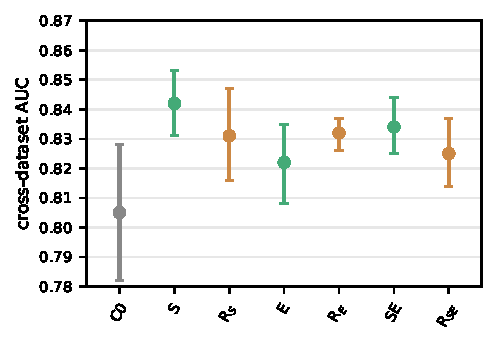
\includegraphics[width=0.78\columnwidth]{fig_bert_controls.pdf}
\caption{Archived protocol: DistilBERT cross-dataset AUC (mean, 95\% interval over eight seeds): baseline (gray), real masking (green) and size-matched random deletion (orange). Real masking is not distinguishable from random deletion; the vertical axis starts at 0.78.}
\label{fig:bertctl}
\end{figure}

\subsection{Matched controls under length matching, and a second transformer}\label{sec:matched}
Two gaps remained after the analyses above: S+L+E had no matched random control, and the transformer result rested on a single model. We closed both. Two conditions were added, L+R$_E$ and L+R$_{SE}$, which apply length matching and then delete as many random words as entity masking (respectively source-plus-entity masking) removes; they are the matched controls of L+E and S+L+E. RoBERTa-base was trained with the DistilBERT recipe (Section~\ref{sec:models}) on the same samples and eight seeds. The new conditions were run for all three models. A seed-0 re-run of conditions C0 and L with the multi-GPU runner used for the new cells reproduced the archived DistilBERT results exactly (AUC, F1, accuracy and AP, difference 0.0 in all 18 cells), so archived and new cells are directly comparable.

\paragraph{Pooled results.}
Table~\ref{tab:matched_pooled} gives the pooled contrasts. For TF-IDF, entity masking beats its matched random control also after length matching: L+E exceeds L+R$_E$ by 0.020 [0.015, 0.024] in all eight seeds, and S+L+E exceeds L+R$_{SE}$ by 0.010 [0.004, 0.016] (seven of eight seeds). For neither transformer does targeted removal beat matched random deletion. For DistilBERT the differences are $-0.013$ [$-0.024$, $-0.001$] and $-0.008$ [$-0.014$, $-0.001$] (seven of eight seeds each); for RoBERTa they are $-0.004$ and $-0.001$, with intervals that include zero. Random deletion alone moves the models in different directions and by different amounts: it lowers TF-IDF cross-dataset AUC by 0.012 [0.007, 0.017] (R$_{SE}$ against C0, eight of eight seeds), raises DistilBERT by 0.020 [$-$0.001, 0.042], and raises RoBERTa by 0.102 [0.081, 0.122] (eight of eight). For RoBERTa the baseline cross-dataset AUC is 0.813, and masking raises it by 0.069 (S) to 0.092 (S+L+E), but random deletion raises it more (R$_{SE}$ +0.102). Adding random deletion on top of length matching raises RoBERTa by 0.117 [0.088, 0.146] and DistilBERT by 0.019 [0.003, 0.035], and does nothing for TF-IDF ($-0.003$ [$-0.009$, 0.003]).

\begin{table}[t]
\caption{Archived protocol: Matched-control contrasts in cross-dataset AUC, pooled over the six ordered pairs: mean, 95\% interval over eight seeds, and number of seeds agreeing in sign with the mean. Bold: interval excludes zero (before rounding). Above the rule: the six contrasts treated as primary; below: exploratory.}\label{tab:matched_pooled}
\footnotesize
\adjustbox{max width=\linewidth}{\begin{tabular}{@{}lccc@{}}
\toprule
Contrast & TF-IDF & DistilBERT & RoBERTa \\
\midrule
S $-$ R$_S$ & \textbf{$-$0.014 [$-$0.019, $-$0.009] (8/8)} & +0.011 [$-$0.009, +0.030] (5/8) & \textbf{$-$0.029 [$-$0.042, $-$0.015] (7/8)} \\
E $-$ R$_E$ & \textbf{+0.020 [+0.016, +0.024] (8/8)} & $-$0.010 [$-$0.025, +0.005] (5/8) & $-$0.008 [$-$0.034, +0.018] (5/8) \\
S+E $-$ R$_{SE}$ & \textbf{+0.016 [+0.010, +0.022] (8/8)} & +0.009 [$-$0.002, +0.020] (6/8) & $-$0.008 [$-$0.018, +0.003] (6/8) \\
L $-$ C0 & \textbf{+0.034 [+0.028, +0.039] (8/8)} & +0.018 [$-$0.006, +0.043] (6/8) & $-$0.024 [$-$0.057, +0.009] (6/8) \\
\midrule
L+E $-$ L+R$_E$ & \textbf{+0.020 [+0.015, +0.024] (8/8)} & \textbf{$-$0.013 [$-$0.024, $-$0.001] (7/8)} & $-$0.004 [$-$0.023, +0.016] (5/8) \\
S+L+E $-$ L+R$_{SE}$ & \textbf{+0.010 [+0.004, +0.016] (7/8)} & \textbf{$-$0.008 [$-$0.014, $-$0.001] (7/8)} & $-$0.001 [$-$0.013, +0.011] (5/8) \\
L+R$_{SE}$ $-$ L & $-$0.003 [$-$0.009, +0.003] (4/8) & \textbf{+0.019 [+0.003, +0.035] (7/8)} & \textbf{+0.117 [+0.088, +0.146] (8/8)} \\
R$_{SE}$ $-$ C0 & \textbf{$-$0.012 [$-$0.017, $-$0.007] (8/8)} & +0.020 [$-$0.001, +0.042] (6/8) & \textbf{+0.102 [+0.081, +0.122] (8/8)} \\
\bottomrule
\end{tabular}
}
\end{table}

\paragraph{Model differences.}
Table~\ref{tab:model_diff} compares the models directly through paired seed-wise differences, as in Section~\ref{sec:stats}. The entity-specific advantage of TF-IDF over DistilBERT holds with length matching (L+E against L+R$_E$: $D=+0.032$ [0.019, 0.045], eight of eight seeds), extending the earlier result without length matching ($+0.030$). The two transformers do not differ clearly on the targeted-removal contrasts (all intervals of DistilBERT $-$ RoBERTa include zero except S against R$_S$ and the random-deletion contrasts): source masking is worse than random deletion for RoBERTa but not for DistilBERT ($D=+0.039$ [0.017, 0.062], eight of eight). The effect of random deletion itself differs strongly between transformers, with RoBERTa gaining about 0.08 AUC more than DistilBERT from R$_{SE}$ (DistilBERT $-$ RoBERTa $-0.081$ [$-0.113$, $-0.050$], eight of eight seeds).

\begin{table}[t]
\caption{Archived protocol: Paired seed-wise differences in the pooled contrast between two models (mean, 95\% interval over eight seeds, seeds agreeing in sign). Bold: interval excludes zero.}\label{tab:model_diff}
\footnotesize
\adjustbox{max width=\linewidth}{\begin{tabular}{@{}lccc@{}}
\toprule
Contrast & TF-IDF $-$ DistilBERT & TF-IDF $-$ RoBERTa & DistilBERT $-$ RoBERTa \\
\midrule
S $-$ R$_S$ & \textbf{$-$0.025 [$-$0.043, $-$0.006] (8/8)} & \textbf{+0.015 [+0.000, +0.029] (7/8)} & \textbf{+0.039 [+0.017, +0.062] (8/8)} \\
E $-$ R$_E$ & \textbf{+0.030 [+0.014, +0.046] (8/8)} & \textbf{+0.028 [+0.000, +0.056] (7/8)} & $-$0.002 [$-$0.020, +0.016] (4/8) \\
S+E $-$ R$_{SE}$ & +0.007 [$-$0.002, +0.017] (5/8) & \textbf{+0.024 [+0.010, +0.038] (7/8)} & +0.016 [$-$0.001, +0.034] (6/8) \\
L $-$ C0 & +0.015 [$-$0.007, +0.038] (6/8) & \textbf{+0.058 [+0.024, +0.091] (7/8)} & +0.042 [$-$0.002, +0.087] (6/8) \\
\midrule
L+E $-$ L+R$_E$ & \textbf{+0.032 [+0.019, +0.045] (8/8)} & \textbf{+0.023 [+0.004, +0.042] (6/8)} & $-$0.009 [$-$0.036, +0.018] (4/8) \\
S+L+E $-$ L+R$_{SE}$ & \textbf{+0.018 [+0.007, +0.029] (7/8)} & \textbf{+0.011 [+0.002, +0.021] (7/8)} & $-$0.007 [$-$0.022, +0.009] (6/8) \\
L+R$_{SE}$ $-$ L & \textbf{$-$0.022 [$-$0.039, $-$0.005] (7/8)} & \textbf{$-$0.120 [$-$0.147, $-$0.093] (8/8)} & \textbf{$-$0.098 [$-$0.130, $-$0.067] (8/8)} \\
R$_{SE}$ $-$ C0 & \textbf{$-$0.032 [$-$0.050, $-$0.014] (7/8)} & \textbf{$-$0.113 [$-$0.133, $-$0.093] (8/8)} & \textbf{$-$0.081 [$-$0.113, $-$0.050] (8/8)} \\
\bottomrule
\end{tabular}
}
\end{table}

\paragraph{Dataset pairs.}
The pooled values for S+L+E hide effects of opposite sign (Table~\ref{tab:matched_pairs}, Fig.~\ref{fig:matched_pairs}). For both transformers, S+L+E beats its matched random control on the two transfers between ISOT and McIntire (DistilBERT +0.046 and +0.083, RoBERTa +0.042 and +0.028) and falls below it on transfers involving the WELFake residual (DistilBERT $-0.021$ to $-0.063$, eight of eight seeds for all four; RoBERTa $-0.015$ to $-0.022$, with three of four intervals excluding zero and ISOT$\rightarrow$residual inconclusive). TF-IDF shows no such split: only McIntire$\rightarrow$ISOT is clearly positive ($+0.049$ [0.035, 0.064]), and the other five pairs are inconclusive. For the entity-only contrast (L+E against L+R$_E$) the DistilBERT negatives on transfers into the residual do not appear for RoBERTa, so only the S+L+E pattern replicates across the two transformers. These pair-level contrasts are exploratory: they are 12 uncorrected contrasts per model, and with eight seeds the smallest attainable exact sign-flip $p$ (0.0078) already exceeds the Holm threshold $0.05/12$. We do not explain the pattern; the data do not separate the contribution of source and entity masking per pair.

\begin{table}[t]
\caption{Archived protocol: Per-pair matched-control contrasts in cross-dataset AUC (mean, 95\% interval over eight seeds, seeds agreeing in sign). Bold: interval excludes zero. Exploratory, uncorrected.}\label{tab:matched_pairs}
\footnotesize
\adjustbox{max width=\linewidth}{\begin{tabular}{@{}lccc@{}}
\toprule
Transfer & TF-IDF & DistilBERT & RoBERTa \\
\midrule
\multicolumn{4}{@{}l}{\textit{S+L+E $-$ L+R$_{SE}$}} \\
ISOT$\rightarrow$McIntire & +0.008 [$-$0.008, +0.025] (6/8) & \textbf{+0.046 [+0.023, +0.069] (8/8)} & \textbf{+0.042 [+0.024, +0.061] (8/8)} \\
ISOT$\rightarrow$residual & +0.002 [$-$0.013, +0.017] (5/8) & \textbf{$-$0.063 [$-$0.082, $-$0.043] (8/8)} & $-$0.022 [$-$0.069, +0.025] (6/8) \\
McIntire$\rightarrow$ISOT & \textbf{+0.049 [+0.035, +0.064] (8/8)} & \textbf{+0.083 [+0.057, +0.109] (8/8)} & \textbf{+0.028 [+0.007, +0.048] (7/8)} \\
McIntire$\rightarrow$residual & $-$0.005 [$-$0.012, +0.002] (6/8) & \textbf{$-$0.021 [$-$0.032, $-$0.010] (8/8)} & \textbf{$-$0.022 [$-$0.033, $-$0.010] (7/8)} \\
residual$\rightarrow$ISOT & +0.014 [$-$0.009, +0.037] (6/8) & \textbf{$-$0.062 [$-$0.089, $-$0.035] (8/8)} & \textbf{$-$0.019 [$-$0.031, $-$0.008] (8/8)} \\
residual$\rightarrow$McIntire & $-$0.007 [$-$0.018, +0.003] (7/8) & \textbf{$-$0.030 [$-$0.043, $-$0.017] (8/8)} & \textbf{$-$0.015 [$-$0.025, $-$0.004] (8/8)} \\
\midrule
\multicolumn{4}{@{}l}{\textit{L+E $-$ L+R$_{E}$}} \\
ISOT$\rightarrow$McIntire & \textbf{+0.014 [+0.001, +0.027] (6/8)} & $-$0.008 [$-$0.045, +0.029] (5/8) & $-$0.039 [$-$0.088, +0.011] (6/8) \\
ISOT$\rightarrow$residual & $-$0.003 [$-$0.017, +0.010] (4/8) & \textbf{$-$0.079 [$-$0.127, $-$0.030] (8/8)} & +0.043 [$-$0.020, +0.105] (7/8) \\
McIntire$\rightarrow$ISOT & \textbf{+0.072 [+0.061, +0.083] (8/8)} & +0.038 [$-$0.000, +0.077] (7/8) & $-$0.017 [$-$0.048, +0.013] (6/8) \\
McIntire$\rightarrow$residual & +0.000 [$-$0.007, +0.007] (5/8) & \textbf{$-$0.016 [$-$0.024, $-$0.008] (8/8)} & +0.003 [$-$0.016, +0.023] (3/8) \\
residual$\rightarrow$ISOT & \textbf{+0.029 [+0.013, +0.044] (8/8)} & $-$0.012 [$-$0.052, +0.028] (3/8) & $-$0.008 [$-$0.034, +0.017] (5/8) \\
residual$\rightarrow$McIntire & +0.007 [$-$0.001, +0.014] (6/8) & +0.002 [$-$0.018, +0.021] (5/8) & $-$0.003 [$-$0.013, +0.008] (3/8) \\
\bottomrule
\end{tabular}
}
\end{table}

\begin{figure}[t]
\centering
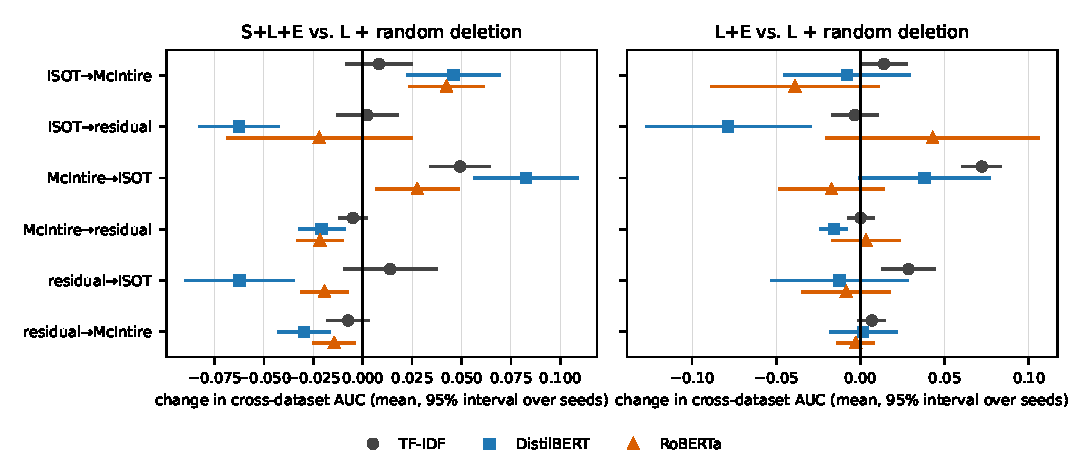
\includegraphics[width=\linewidth]{fig_matched_pairs.pdf}
\caption{Archived protocol: Per-pair matched-control contrasts in cross-dataset AUC for the three models (mean and 95\% interval over eight seeds). Left: S+L+E minus length matching plus random deletion of the same size; right: L+E minus length matching plus random deletion. Points to the right of zero mean targeted removal transfers better than random deletion.}\label{fig:matched_pairs}
\end{figure}

\paragraph{Multiplicity.}
Over the six primary contrasts, the exact paired sign-flip $p$-values of TF-IDF are 0.0078 (five contrasts) and 0.0156 (S+L+E against L+R$_{SE}$), giving Holm-adjusted $p=0.047$ for all six; none of the six contrasts survives Holm correction for DistilBERT or RoBERTa (smallest adjusted $p=0.094$ for both). This family was defined after the earlier exploratory results had been seen, and the sign-flip $p$-values describe stability under resampling within one fixed document universe, so we treat the adjusted values as descriptive and not as confirmatory evidence.

\setlength{\bibsep}{0.6em}
\bibliography{refs}
\end{document}
